\chapter{Géométrie plane} \label{G9}

\bigskip

\begin{figure}[h]
   \centering
      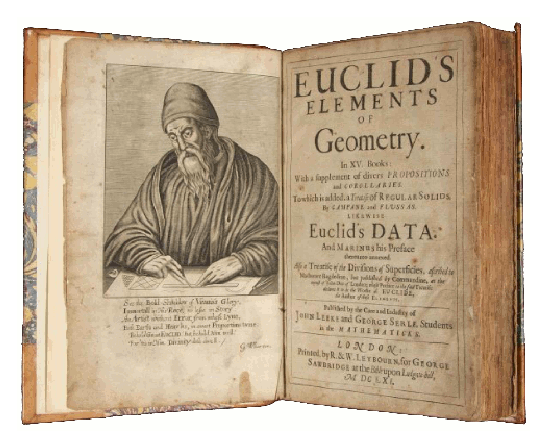
\includegraphics[height=6cm]{Geometrie/Images/G9_intro_Euclide}
   \caption{Euclid's elements of Geometry, 1661, John Leeke, Georges Searle}
\end{figure}

\begin{prerequis}[Un peu d'histoire]
   L'objet de la géométrie (du grec \textit{géo} : terre ; \textit{metria} : mesure) concerne la connaissance des relations spatiales. Avec l'arithmétique, elle constitue, dans l'antiquité, l'un des deux domaines des mathématiques les plus recherchés. Si les grecs peuvent être considérés comme les fondateurs de la géométrie en tant que science et discipline mathématique, de nombreuses connaissances en géométrie, nécessaires à la topographie, l'architecture, l'astronomie et l'agriculture, ont précédé la civilisation grecque. Les premières notions de géométrie reconnues remontent à 3\,000 ans av. J.-C., du temps de l'Égypte ancienne, de l'ancienne civilisation hindoue et des babyloniens. \\
   Pour les mathématiciens de la Grèce antique, la géométrie est au c\oe ur des sciences. La tradition attribue à \textbf{Thalès} l'introduction en Grèce de la géométrie égyptienne. Par rapport à leurs prédécesseurs, les Grecs étudient de nouvelles figures, dont des courbes, surfaces et solides. Mais surtout, ils innovent au niveau de la méthode, en généralisant des lois à partir des nombreuses règles empiriques connues depuis longtemps. La géométrie grecque est marquée par deux écoles : celle de \textbf{Pythagore} à l'école de Crotone, et celle d'\textbf{Euclide} à l'école d'Alexandrie. Les travaux de cette dernière, qui connut trois représentant exceptionnels que sont Euclide, \textbf{Archimède} et \textbf{Appolonius} débouchent sur une \oe uvre qui pendant plus de 20 siècles servit de base à toute étude géométrique : \textit{les éléments}. La géométrie classique, issue de celle d'Euclide, est basée sur des constructions obtenues à l'aide de droites et de cercles, c'est à dire élaborées \og à la règle et au compas \fg{}.
\end{prerequis}

   
\cours

Dans ses livres, {\it Les éléments}, Euclide définit les objets géométriques au 3\up{ième} siècle av. J.-C. Le livre 1 comprend 35 définitions fondamentales de la géométrie euclidienne, comme par exemple :

{\renewcommand{\StringDOCUMENTATION}{Les définitions d'Euclide}
\begin{documentation}
   {\it
   \begin{itemize}
      \item Le {\bf point} est ce dont la partie est nulle ;
      \item une {\bf ligne} est une longueur sans largeur ;
      \item la {\bf ligne droite} est celle qui est également placée entre ses points ;
      \item un {\bf angle} plan est l'inclinaison mutuelle de deux lignes qui se touchent dans un plan, et qui ne sont pas placées dans la même direction ;
      \item un {\bf cercle} est une figure plane comprise par une seule ligne qu'on nomme circonférence, toutes les droites menées à la circonférence d'un des points placé dans cette figure étant égales entre elles. \\ [-8mm]
   \end{itemize}}
\end{documentation}}

\medskip

Attardons nous sur le vocabulaire \og moderne \fg{} de ces objets géométriques ainsi qu'aux constructions géométriques dans le plan euclidien.

\section{Les droites} %%% 1

\subsection{Définition} % A

\begin{definition}[Droite - segment]
   Une \textbf{droite} est une ligne rectiligne, infinie et sans épaisseur. Une \textbf{demi-droite} est une portion de droite limitée d'un seul côté par un point appelé origine. \\
   Un \textbf{segment} est une portion de droite limitée par deux points appelés extrémités.
\end{definition}

\begin{exemple*1}
   \begin{minipage}{6cm}
   {\psset{unit=0.6}
   \begin{pspicture}(0,1.5)(9,6.5)
      \psset{dotsize=8pt,dotstyle=x}
      \psline(4,5)(8,2)
      \psline(1,2)(9,2)
      \psline(2,2)(5,6.5)
      \psdots(2,2)(5,2)(8,2)(4,5)
      \rput[bl](1.7,1.3){A}
      \rput[bl](4.8,1.3){B}
      \rput[bl](7.8,1.3){C}
      \rput[bl](3.7,5.3){D}
   \end{pspicture}} 
   \end{minipage}
   \begin{minipage}{6cm}
   \begin{itemize}
      \item (AC), (AB) et (BC) sont des droites ;
      \item $[$AD) est la demi-droite d'origine A ;
      \item $[$CD$]$ est un segment ;
      \item B $\in$ (AC) mais B $\not\in$ (DC).
   \end{itemize}
   \end{minipage}
\end{exemple*1}

\begin{notation}
   le symbole $\in$ signifie \og appartient à \fg{} et $\not\in$ signifie \og n'appartient pas à \fg.
\end{notation}


\subsection{Position relative de deux droites} % B

\begin{definition}[Droites sécantes]
   Lorsque deux droites ont un point en commun, on dit qu'elles sont \textbf{sécantes}.
\end{definition}

\begin{exemple*1}
   \begin{minipage}{6cm}
   {\psset{unit=0.9}
   \begin{pspicture}(-1,-0.5)(4,2.2)
      \psset{yunit=0.6}
      \rput(0,-0.4){A}
      \rput(4,3.1){B}
      \rput(0,2.4){C}
      \rput(4,0.5){D}
      \rput(1.5,0.8){O}
      \psline(0,0)(4,3.5)
      \psline(0,2)(4,0)
   \end{pspicture}}
   \end{minipage}
   \begin{minipage}{7cm}
      Les droites (AB) et (CD) sont sécantes en O.
   \end{minipage}
\end{exemple*1}

\begin{definition}[Droites perpendiculaires]
   Lorsque deux droites forment un angle droit, on dit qu'elles sont \textbf{perpendiculaires}.
\end{definition}

\begin{exemple*1}
  \begin{minipage}{5cm}
   \begin{pspicture}(-1,0)(4,2)
      {\psset{unit=0.8}
      \psline(0,0)(4,2)
      \psline(2.5,0)(1,3)
      \pspolygon(2,1)(2.25,1.125)(2.125,1.375)(1.875,1.25)
      \equerre{2}{1}{116.5}{1}
      \rput(3.8,1.6){$d$}
      \rput(1.5,2.9){$\Delta$}}
   \end{pspicture}
   \end{minipage}
   \begin{minipage}{7cm}
      Les deux droites $d$ et $\Delta$ sont perpendiculaires. \\
      On peut le constater grâce à une équerre.
   \end{minipage}
\end{exemple*1}

\begin{methode}[Construction d'une perpendiculaire avec un compas]
Pour tracer la droite $\Delta$ perpendiculaire à la droite $d$ en A, on effectue deux arcs de cercle sur la droite $d$ en plaçant la pointe du compas en A. Ces arcs définissent deux points sur $d$. À partir de ces points, on effectue deux fois deux arcs de cercle de part et d'autre de $d$ en gardant le même écartement, puis on trace la droite $\Delta$ passant par les deux intersections formées par les arcs de cercle.
\exercice
\begin{pspicture}(-1,-1)(3.5,2.5)
      \psline(0,0)(4,1)
      \psdot(2,0.5)
      \rput(2.35,0.25){A}
      \rput(3.6,1.2){$d$}
   \end{pspicture} 
\correction    
   \begin{pspicture}(0,-1)(3.5,2.5)
      \psline(0,0)(4,1)
      \psdot(2,0.5)
      \rput(2.35,0.25){A}
      \rput(3.6,1.2){$d$}
      \psarc[linecolor=A1](2,0.5){1.5}{0}{30}
      \psarc[linecolor=A1](2,0.5){1.5}{180}{210}
   \end{pspicture}      
   \begin{pspicture}(-1,-1)(3.5,2.5)
      \psline(0,0)(4,1)
      \psdot(2,0.5)
      \rput(2.35,0.25){A}
      \psarc[linecolor=A1](2,0.5){1.5}{0}{30}
      \psarc[linecolor=A1](2,0.5){1.5}{180}{210}
      \psdot(3.46,0.86)
      \psarc[linecolor=B2](3.46,0.86){2.5}{130}{150}
      \psarc[linecolor=B2](3.46,0.86){2.5}{240}{260}
      \psarc[linecolor=B2](0.54,0.14){2.5}{-50}{-30}
      \psarc[linecolor=B2](0.54,0.14){2.5}{60}{80}
      \psline[linecolor=B2,linewidth=0.05](2.6,-1.8)(1.29,3.3)
      \rput(3.6,1.2){$d$}
      \rput(1,3){\textcolor{B2}{$\Delta$}}      
   \end{pspicture}
\end{methode}

\begin{definition}[Droites parallèles]
   Lorsque deux droites ne se coupent pas, on dit qu'elles sont \textbf{parallèles}.
\end{definition}

\begin{exemple*1}
   \begin{minipage}{6cm}
   \begin{pspicture}(-1.5,0)(4,2)
      {\psset{unit=0.8}
      \psline(0,0)(4,2)
      \psline(-0.5,0.7)(3.5,2.7)
      \rput(3.8,1.4){$d$}
      \rput(3.4,2.3){$d'$}}
   \end{pspicture}
   \end{minipage}
   \begin{minipage}{7cm}
      Les deux droites $d$ et $d'$ sont parallèles.
   \end{minipage}
\end{exemple*1}

\begin{methode}[Construction d'une parallèle à la règle et à l'équerre]
Pour tracer la parallèle $d'$ à $d$ passant par A, on trace la perpendiculaire $\Delta$ à $d$ passant par A, puis on trace la perpendiculaire $d'$ à $\Delta$ passant par A.
\exercice
\begin{pspicture}(-1,0)(3.5,3)
      \psline(0,0)(4,1)
      \psdot(0.65,1.69)
      \rput(0.55,1.45){A}
      \rput(3.6,1.2){$d$}
   \end{pspicture}  
\correction   
   \begin{pspicture}(0,0)(3.5,3)
      \psline(0,0)(4,1)
      \psdot(0.65,1.69)
      \rput(0.55,1.45){A}
      \psline[linecolor=A1,linewidth=0.05](1.135,-0.3)(0.34,2.9)
      \equerre{1.02}{0.28}{14}{1}
      \regle{0}{-0.25}{14}{1}
      \rput(3.6,1.2){$d$}
      \rput(0.7,2.7){\textcolor{A1}{$\Delta$}}
   \end{pspicture} 
   \begin{pspicture}(-1,0)(3.5,3)
      \psline(0,0)(4,1)
      \psdot(0.65,1.69)
      \rput(0.55,1.45){A}
      \psline[linecolor=B2,linewidth=0.05](-0.2,1.5)(3.8,2.5)
      \equerre{0.68}{1.68}{-76}{1}
      \psline[linecolor=A1,linewidth=0.05](1.135,-0.3)(0.34,2.9)
      \rput(3.6,1.2){$d$}
      \rput(0.7,2.7){\textcolor{A1}{$\Delta$}}
      \rput(3.5,2.85){\textcolor{B2}{$d'$}}
      \regle{0.25}{2}{-76}{1}
   \end{pspicture} 
\end{methode}


\subsection{Médiatrice} % C

\begin{definition}[Médiatrice d'un segment]
   La \textbf{médiatrice} d'un segment est la droite perpendiculaire à ce segment et qui passe par son milieu.
\end{definition}

\begin{methode}[Construction de la médiatrice d'un segment à la règle et au compas]
Pour tracer la médiatrice du segment [AB], on choisit un écartement au compas et on trace deux arcs de cercle à partir de A et de B de part et d'autre du segment [AB]. On trace la droite passant par les deux points formés par l'intersection des arcs de cercle.
\exercice
   \begin{pspicture}(-1,-0.25)(4,3.5)
      \pstGeonode[PosAngle=180,linecolor=A1](1,3){A}
       \pstGeonode[PointSymbol=none,PointName=none](0,0){C}(4,3){D}
       \pstOrtSym[linecolor=A1]{C}{D}{A}[B] 
       \pstLineAB{A}{B} 
   \end{pspicture}
\correction
   \begin{pspicture}(0,-0.25)(4,3.5)
       \pstGeonode[PosAngle=180,linecolor=A1](1,3){A}
       \pstGeonode[PointSymbol=none,PointName=none](0,0){C}(4,3){D}
       \psarc[linecolor=A1,linestyle=dashed](1,3){2}{260}{300}
       \psarc[linecolor=A1,linestyle=dashed](1,3){2}{320}{360}
       \pstOrtSym[linecolor=A1]{C}{D}{A}[B] 
       \pstLineAB{A}{B}
       \psarc[linecolor=A1,linestyle=dashed](3.18,0.16){2}{80}{120}
       \psarc[linecolor=A1,linestyle=dashed](3.18,0.16){2}{140}{175}
   \end{pspicture} 
   \begin{pspicture}(0,-0.25)(4,3.5)
      \pstGeonode[PosAngle=180,linecolor=A1](1,3){A}
      \pstGeonode[PointSymbol=none,PointName=none](0,0){C}(4,3){D}
      \psarc[linecolor=A1,linestyle=dashed](1,3){2}{260}{300}
      \psarc[linecolor=A1,linestyle=dashed](1,3){2}{320}{360}
      \pstOrtSym{C}{D}{A}[B] 
      \pstLineAB{A}{B}
      \psarc[linecolor=A1,linestyle=dashed](3.18,0.16){2}{80}{120}
      \psarc[linecolor=A1,linestyle=dashed](3.18,0.16){2}{140}{175} 
      \pstMediatorAB[CodeFig=true,PointName=none,PointSymbol=none]{A}{B}{I}{F}  
      \pstMediatorAB[PointName=none,PointSymbol=none]{B}{A}{I}{E}     
      \pstLineAB[linecolor=B2,linewidth=0.05]{E}{F} 
   \end{pspicture} 
\end{methode}


\subsection{Hauteur} %%% D 

\begin{minipage}{14cm}
   \begin{definition}[Distance d'un point à une droite]
      La distance d'un point $A$ à la droite $(d)$ est la plus courte distance séparant le point A d'un point de $(d)$.
   \end{definition}
   \smallskip
   \begin{propriete}
      La distance d'un point $A$ à la droite $(d)$ est égale à la longueur du segment $[AH]$ où $H$ est le pied de la perpendiculaire à $(d)$ passant par $A$.
   \end{propriete}
\end{minipage}
\begin{minipage}{6cm}
   {\psset{unit=0.7}
   \begin{pspicture}(2.5,1.5)(6,6)
      \pstGeonode[PointSymbol=+,PosAngle={90,-45}](1,5){A}(4,4){P}(2,2){N}(5,5){Q}(3,3){H}
      \pstLineAB[nodesep=-10mm]{N}{Q}
      \pstLineAB[linecolor=A1]{A}{N}
      \pstLineAB[linecolor=B1]{A}{H}
      \pstLineAB[linecolor=A1]{A}{P}
      \pstLineAB[linecolor=A1]{A}{Q}
      \pstRightAngle[linecolor=B1]{Q}{H}{A}
      \rput(5.5,6.5){$(d)$} 
   \end{pspicture}}
\end{minipage}

\begin{definition}[Hauteurs d'un triangle]
   Les \textbf{hauteurs} d'un triangle sont les hauteurs relatives aux sommets du triangle, c'est-à-dire les trois droites perpendiculaires aux côtés qui passent par le sommet opposé.
\end{definition}

\begin{pspicture}(-0.5,-0.5)(4,4)
   \psset{CodeFig=true, PointSymbol=none,RightAngleSize=0.2}
   \pstTriangle{A}(4.5,0){B}(1.5,3){C}
   \pstProjection[PointName=none,CodeFigColor=B1]{B}{C}{A}
   \pstLabelAB[offset=-0.3,npos=0.56]{A}{A'}{\footnotesize \textcolor{B1}{hauteur issue de A}}
   \pstLineAB[linecolor=A1,linewidth=0.5mm]{C}{B}
   \pstLabelAB{C}{B}{\footnotesize \textcolor{A1}{base relative à la hauteur issue de A}}
\end{pspicture}
\begin{pspicture}(-1.5,-0.5)(4,4)
   \psset{CodeFig=true, PointSymbol=none,RightAngleSize=0.2}
   \pstTriangle{A}(4.5,0){B}(1.5,3){C}
   \pstProjection[PointName=none,CodeFigColor=B1]{C}{A}{B}
   \pstLabelAB[offset=-0.3,npos=0.4]{B'}{B}{\footnotesize \textcolor{B1}{hauteur issue de B}}
   \pstLineAB[linecolor=A1,linewidth=0.5mm]{A}{C}
   \pstLabelAB[offset=0.5]{A}{C}{\footnotesize \textcolor{A1}{base relative à la hauteur issue de B}}
\end{pspicture}
\begin{pspicture}(-1.5,-0.5)(4,4)
   \psset{CodeFig=true, PointSymbol=none,RightAngleSize=0.2}
   \pstTriangle{A}(4.5,0){B}(1.5,3){C}
   \pstProjection[PointName=none,CodeFigColor=B1]{B}{A}{C}
   \pstLabelAB[offset=-0.3,npos=0.45]{C'}{C}{\footnotesize \textcolor{B1}{hauteur issue de C}}
   \pstLineAB[linecolor=A1,linewidth=0.5mm]{A}{B}
   \pstLabelAB[offset=-0.3]{A}{B}{\footnotesize \textcolor{A1}{base relative à la hauteur issue de C}}
\end{pspicture}


Pour tracer la hauteur dans un triangle issue d'un sommet, on trace la droite passant par ce sommet et perpendiculaire au côté opposé.


\section{Les angles} %%% 2

\subsection{Mesurer un angle} % A

\begin{definition}[Angle]
   Un \textbf{angle} est une portion du plan délimitée par deux droites.
\end{definition}

\begin{pspicture}(-6,-0.3)(4,2.5)
      {\psset{yunit=0.5}
      \rput(0,-0.3){A}
      \rput(4,3.6){B}
      \rput(0,2.3){C}
      \rput(4,0.3){D}
      \rput(1.4,1){O}
      \psline(0,0)(4,4)
      \psline(0,2)(4,0)
      \psarc[linecolor=A1](1.4,1.4){1}{-17}{27}
      \psline[linecolor=B2]{->}(-1,1.1)(1.3,1.3)
      \rput(-1.8,1.3){\textcolor{B2}{sommet}}
      \rput(3.5,1.7){\textcolor{A1}{angle $\widehat{BOD}$}}}
   \end{pspicture}

Angles particuliers :

\begin{tabular}{C{2}C{3}C{3}C{4}C{4}}
   \begin{pspicture}(0,0)(2,0)
      \psline(0,0)(2,0)
      \psdots(0,0)
   \end{pspicture}
   &
   \begin{pspicture}(0,0)(3,1.5)
      \psline(0,0)(3,0)
      \psline(0,0)(3,1.5)
      \psarc[linecolor=A1](0,0){1}{0}{27}
      \psdots(0,0)
   \end{pspicture}
   &
   \begin{pspicture}(0,0)(3,1.5)
      \pspolygon[linecolor=A1](0,0)(0.5,0)(0.5,0.5)(0,0.5)
      \psline(0,0)(3,0)
      \psline(0,0)(0,1.5)
      \psdots(0,0)
   \end{pspicture}
   &
   \begin{pspicture}(-2,0)(2,1.5)
      \psline(0,0)(2,0)
      \psline(0,0)(-2,1.5)
      \psarc[linecolor=A1](0,0){0.5}{0}{145}
      \psdots(0,0)
   \end{pspicture}
   &
   \begin{pspicture}(-2,0)(2,1)
      \psline(-2,0)(2,0)
      \psdots(0,0)
      \psarc[linecolor=A1](0,0){0.5}{0}{180}
   \end{pspicture} \\
      angle nul & angle aigu & angle droit & angle obtus & angle plat \\
\end{tabular}

\begin{definition}[Rapporteur - degré]
   Un \textbf{rapporteur} est un instrument de mesure permettant de mesurer des angles. \\
   L'unité de mesure utilisée au collège est le \textbf{degré}.
\end{definition}

\begin{center}
\begin{pspicture}(-3,-0.5)(5,3.5)
   {\psset{unit=0.75}
      \rapporteur{0}{0}{0}{1}
      \psline[linewidth=0.1](6,3.46)(0,0)(6,0)
      \rput(5,1.4){\textcolor{B2}{\small 0 extérieur}}
      \psline[linecolor=B2,arrowsize=0.3,linestyle=dashed]{<-}(3.75,0)(4.75,1)
      \rput(4,4.4){\textcolor{A1}{\small lecture de l'angle : $30^\circ$}}
      \psline[linecolor=A1,arrowsize=0.3,linestyle=dashed]{<-}(3.75;30)(4,4)}
   \end{pspicture} 
\end{center}

%\begin{methode}[Déterminer la mesure d'un angle avec un rapporteur]
%   Pour déterminer la mesure en degré de l'angle $\widehat{\text{BAC}}$:
%\begin{itemize}
%      \item on commence par placer le centre du rapporteur sur le point A, sommet de l'angle ;
%      \item on fait pivoter le rapporteur autour de son centre de façon à ce que l'un des côtés de l'angle passe par l'une des deux graduations \og 0 \fg{} ;
%      \item on lit la graduation du même côté que le \og 0 \fg{} choisi sur le deuxième côté de l'angle.
%   \end{itemize}
%\exercice
%   \begin{pspicture}(-1,-0.5)(5,3.4)
%      {\psset{unit=0.8}
%      \rput(5,0.4){B}
%      \rput(0,-0.35){A}
%      \psdots(5,0)
%      \rput(5,3.3){C}
%      \psdots(5,2.89)
%      \psline[linewidth=0.1](6,3.46)(0,0)(6,0)}
%   \end{pspicture}   
%\correction
%   \begin{pspicture}(-3.5,-0.5)(8,3.4)
%   {\psset{unit=0.8}
%      \rapporteur{0}{0}{0}{1}
%      \rput(5,0.4){B}
%      \rput(0,-0.35){A}
%      \psdots(5,0)
%      \rput(5,3.3){C}
%      \psdots(5,2.89)
%      \psline[linewidth=0.1](6,3.46)(0,0)(6,0)
%      \rput(5,1.4){\textcolor{B2}{\small 0 extérieur}}
%      \psline[linecolor=B2,arrowsize=0.3,linestyle=dashed]{<-}(3.75,0)(4.75,1)
%      \rput(4,4.4){\textcolor{A1}{\small lecture de l'angle : $30^\circ$}}
%      \psline[linecolor=A1,arrowsize=0.3,linestyle=dashed]{<-}(3.75;30)(4,4)}
%   \end{pspicture}   
%\end{methode}

%\begin{methode}[Construire un angle de mesure donnée avec un rapporteur]
%   Pour tracer un angle $\widehat{\text{BAC}}$ dont on connait la mesure :
%   \begin{itemize}
%      \item on commence par tracer le segment [AB] par exemple,
%      \item on place le centre du rapporteur sur le point A, sommet de l'angle ;
%      \item on fait pivoter le rapporteur autour de son centre de façon à ce que le segment [AB] passe par l'une des deux graduations \og $0$ \fg ;
%      \item on lit la graduation correspondant à la mesure souhaitée du même côté que le \og $0$ \fg{} choisi ;
%      \item on marque au crayon la mesure sur le bord du rapporteur ;
%      \item on ôte le rapporteur et on trace [AC], le deuxième côté de l'angle.
%   \end{itemize}
%\exercice   
%   \begin{pspicture}(1,-0.5)(8,4)
%   {\psset{unit=0.8}
%      \rapporteur{6}{0}{0}{1}
%      \rput(6,-0.4){A}
%      \rput(1,-0.4){B}
%      \psdots(6,0)(1,0)
%      \psline[linewidth=0.1](1,0)(6,0)
%      \rput(5,1){\textcolor{B2}{$0$ intérieur}}
%      \psline[linecolor=B2,arrowsize=0.3,linestyle=dashed]{<-}(3.5,0)(4.5,0.7)
%      \rput(11,3.2){\textcolor{A1}{\small marquage de l'angle :}}
%      \rput(11,2.7){\textcolor{A1}{\small $140^\circ$}}      
%      \psline[linecolor=A1,arrowsize=0.3,linestyle=dashed]{<-}(7.9,1.6)(9,3)  
%      \psdot[linecolor=A1,linewidth=0.1](7.9,1.6)}
%   \end{pspicture}
%\correction
%   \begin{pspicture}(-0.5,-0.5)(8,4)
%   {\psset{unit=0.8}
%      \rput(6,-0.4){A}
%      \rput(1,-0.4){B}
%      \psdots(6,0)(1,0)
%      \psdot[linecolor=A1,linewidth=0.1](7.9,1.6)
%      \psline[linewidth=0.1](1,0)(6,0)
%      \psline[linewidth=0.1,linecolor=A1](6,0)(9,2.5)
%      \rput(7.9,1){\textcolor{A1}{C}}
%      \psarc[linecolor=A1](6,0){1}{40}{180}
%      \rput(5.8,1.5){\textcolor{A1}{$140^\circ$}}}
%   \end{pspicture}
%\end{methode}
%
%\begin{remarque}
%   lorsque le segment tracé est trop court pour pouvoir lire l'angle ou placer correctement le rapporteur, il suffit de le prolonger.
% \end{remarque}

\subsection{Angles particuliers} % B

\begin{definition}[Angles adjacents, complémentaires et supplémentaires]
   \begin{itemize}
      \item Deux angles sont \textbf{adjacents} s'ils ont même sommet, un côté commun et s'ils sont situés de part et d'autre de ce côté commun.
      \item Deux angles sont \textbf{complémentaires} si la somme de leurs mesures est de $90^{\circ}$.
      \item Deux angles sont \textbf{supplémentaires} si la somme de leurs mesures est de $180^{\circ}$. \\ [-8mm]
   \end{itemize}
\end{definition}

\begin{center}
{\psset{unit=0.9}
\begin{pspicture}(0,0)(4,2.5)
   \psline(0,0)(4,0)
   \psline(0,0)(4,2)
   \psline(0,0)(0.67,2)
   \psarc[linecolor=B2,doubleline=true](0,0){1}{0}{25}
   \psarc[linecolor=A1](0,0){0.7}{28}{73}
   \rput(2,-0.5){angles adjacents}
\end{pspicture}
\begin{pspicture}(-1,0)(4,2.5)
   \psline(0,0)(4,0)
   \psline(0,0)(4,2)
   \psline(0,0)(0,2)
   \psarc[linecolor=B2,doubleline=true](0,0){1}{0}{25}
   \psarc[linecolor=A1](0,0){0.7}{28}{90}
   \rput(2,-0.5){angles complémentaires}
\end{pspicture}
\begin{pspicture}(-3,0)(4,2.5)
   \psline(-2,0)(4,0)
   \psline(0,0)(4,2)
   \psarc[linecolor=B2,doubleline=true](0,0){1}{0}{25}
   \psarc[linecolor=A1](0,0){0.7}{28}{180}
   \rput(1,-0.5){angles supplémentaires}
\end{pspicture}}
\end{center}

\pagebreak

\begin{minipage}{8cm}
On considère la configuration suivante :
\end{minipage}
\begin{minipage}{8cm}
\begin{pspicture}(0,-0.5)(6,4)
   \psline(0,1.5)(6,0.5)
   \psline(1,3)(6,3)
   \psline(1,0)(5,4)
   \psarc[linecolor=B2,doubleline=true](4,3){0.7}{0}{45}
   \rput(5,3.4){\textcolor{B2}{$A_2$}}
   \psarc[linecolor=B2,doubleline=true](4,3){0.7}{180}{225}
   \rput(3,2.5){\textcolor{B2}{$A_4$}}
   \psarc[linecolor=A1](4,3){0.5}{45}{180}
   \rput(3.7,3.8){\textcolor{A1}{$A_1$}}
   \psarc[linecolor=A1](4,3){0.5}{225}{0}
   \rput(4.35,2.25){\textcolor{A1}{$A_3$}}
   \psarc[linecolor=B2,doubleline=true](2.15,1.15){0.7}{-10}{45}
   \rput(3.2,1.4){\textcolor{B2}{$B_2$}}
   \psarc[linecolor=B2,doubleline=true](2.15,1.15){0.7}{170}{225}
   \rput(1.1,0.7){\textcolor{B2}{$B_4$}}
   \psarc[linecolor=A1](2.15,1.15){0.5}{45}{170}
   \rput(1.8,1.9){\textcolor{A1}{$B_1$}}
   \psarc[linecolor=A1](2.15,1.15){0.5}{225}{-10}
   \rput(2.4,0.3){\textcolor{A1}{$B_3$}}
\end{pspicture}
\end{minipage}

\begin{definition}[Angles opposés, correspondants, alternes-internes et externes]
   \begin{itemize}
      \item Les angles $A_2$ et $A_4$, $A_1$ et $A_3$, $B_2$ et $B_4$, $B_1$ et $B_3$ sont des angles \textbf{opposés par le sommet}.
      \item Les angles $A_1$ et $B_1$ ; $A_2$ et $B_2$ ; $A_3$ et $B_3$ ; $A_4$ et $B_4$ sont des angles \textbf{correspondants}.
      \item Les angles $A_4$ et $B_2$ ; $A_3$ et $B_1$ sont des angles \textbf{alternes-internes}.
      \item Les angles $A_1$ et $B_3$ ; $A_2$ et $B_4$ sont des angles \textbf{alternes-externes}. \\ [-8mm]
   \end{itemize}
\end{definition}

\begin{exemple*1}
\ \\ [-2mm]
\begin{minipage}{9cm}
   On considère la figure ci-contre pour laquelle les droites $d$ et $d'$ sont parallèles et la droite $\Delta$ est perpendiculaire à $d$.
   \begin{itemize}
      \item les angles $\widehat{ABC}$ et $\widehat{DBE}$ sont opposés par le sommet ;
      \item les angles $\widehat{BCF}$ et $\widehat{DBE}$ sont des angles correspondants ;
      \item les angles $\widehat{BCA}$ et $\widehat{BCF}$ sont complémentaires ;
      \item les angles $\widehat{DBA}$ et $\widehat{DBE}$ sont supplémentaires. \\ [-10mm]
   \end{itemize}
   \end{minipage}
   \begin{minipage}{7cm}
   {\psset{xunit=0.8,yunit=0.7}
   \begin{pspicture}(-3,0)(4,5)
      \psline(-1.5,0)(4,0)
      \psline(-1.5,3.46)(4,3.46)
      \psline(0,-1)(0,4.5)
      \psline(-0.5,-0.865)(3,5.19)
      \rput(-0.25,0.25){C}
      \rput(-0.25,3.71){A}
      \rput(2.25,3.21){B}
      \rput(4,3.71){E}
      \rput(4,0.25){F}
      \rput(3.1,4.8){D}
      \rput(-1.5,0.3){$d'$}
      \rput(-1.5,3.71){$d$}
      \rput(0.3,5){$\Delta$}
      \psarc[linecolor=B2,doubleline=true](0,0){0.5}{0}{60}
      \psarc[linecolor=B2,doubleline=true](2,3.46){0.5}{0}{60}
      \psarc[linecolor=B2,doubleline=true](2,3.46){0.5}{180}{240}
      \psarc[linecolor=A1](0,0){1}{60}{90}
      \psarc[linecolor=J1](2,3.46){0.75}{60}{180}
      \psframe(0,3.46)(0.3,3.76)
   \end{pspicture}}
   \end{minipage}
\end{exemple*1}


%%%%%%%%%%%%%%%%%%%%%%%%%
%\subsection{Bissectrice d'un angle}
%
%\begin{definition}[Bissectrice d'un angle]
%   La \textbf{bissectrice} d'un angle est la droite partageant cet angle en deux angles de même mesure.
%\end{definition}
%
%\begin{methode}[Construction de la bissectrice d'un angle avec un compas]
%    Pour construire la bissectrice de l'angle $\widehat{\text{BAC}}$, à partir de A, on trace deux arcs de cercle sur les segments [AB] et [AC], puis deux arcs de cercle à partir des deux points formés. On trace la droite passant par A et l'intersection des deux derniers arcs de cercle : c'est la bissectrice de l'angle $\widehat{\text{BAC}}$.
%\exercice
%{\psset{unit=0.9}
%   \begin{pspicture}(-1.5,0)(4,4.5)
%       \pstGeonode[PosAngle={180,0,60}](0,0){A}(3,0){B}(2,3.464){C}
%       \pstLineAB{A}{B}
%       \pstLineAB{A}{C}       
%   \end{pspicture}}
%\correction
%{\psset{unit=0.9}
%   \begin{pspicture}(-0.5,0)(4,4.5)
%       \pstGeonode[PosAngle={180,0,60}](0,0){A}(3,0){B}(2,3.464){C}
%       \pstLineAB{A}{B}
%       \pstLineAB{A}{C}
%       \psarc[linecolor=A1,linestyle=dashed](0,0){2.5}{40}{80}
%       \psarc[linecolor=A1,linestyle=dashed](0,0){2.5}{-20}{20}
%       \psarc[linecolor=B2,linestyle=dashed](2.5;0){2.5}{40}{80}
%       \psarc[linecolor=B2,linestyle=dashed](2.5;60){2.5}{-20}{20}
%       \psdot[linecolor=B2,linewidth=0.1](4.33;30)
%   \end{pspicture} 
%   \begin{pspicture}(-0.5,0)(4,4.5)
%       \pstGeonode[PosAngle={180,0,60}](0,0){A}(3,0){B}(2,3.464){C}
%       \pstGeonode[PointName=none,PointSymbol=none](2.625;30){D}
%       \psdot[linecolor=B2,linewidth=0.1](4.33;30)
%       \pstLineAB{A}{B}
%       \pstLineAB{A}{C}
%       \psline[linecolor=B2,linewidth=0.05](0,0)(5;30)
%       \pstMarkAngle[linecolor=A1,Mark=MarkHash,MarkAngleRadius=1,LabelSep=1.7]{B}{A}{D}{\textcolor{A1}{}}
%       \pstMarkAngle[linecolor=A1,Mark=MarkHash,MarkAngleRadius=1,LabelSep=1.7]{D}{A}{C}{\textcolor{A1}{}}       
%    \end{pspicture}} 
%\end{methode}


\section{Les cercles} %%% 3

\begin{definition}[Cercle, rayon, corde, arc]
   \begin{itemize}
      \item Soit O, un point. Le \textbf{cercle} $\mathcal{C}$ de centre O et de {\bf rayon} $r$ est l'ensemble des points situés à une distance $r$ du point O.
      \item Dans un cercle, une \textbf{corde} est un segment reliant deux points du cercle.
      \item Lorsqu'une corde passe par le centre du cercle, on l'appelle un \textbf{diamètre} du cercle.
      \item Une partie du cercle comprise entre deux points est appelé \textbf{arc} de cercle. \\ [-8mm]
   \end{itemize}
\end{definition}

\begin{exemple*1}
\begin{minipage}{5cm}
\begin{pspicture}(-1,0)(3,3.5)
{\psset{unit=0.8}
   \psdots(2,2)
   \psarc(2,2){2}{180}{240}
   \psarc(2,2){2}{240}{180}
   \rput(2,1.6){O}
   \rput(0.4,3.7){$\mathcal{C}$}
   \psline(0,2)(2,2)
   \psdots(0,2)
   \rput(-0.3,2){A}
   \psdots(3,3.7)
   \rput(3.2,4){B}
   \psdots(1,0.3)
   \rput(0.8,-0.2){C}
   \psline(1,0.3)(3,3.7)
   \psline(0,2)(3,3.7)}
\end{pspicture}
\end{minipage}
\begin{minipage}{7cm}
   \begin{itemize}
      \item $[$BC$]$ est un diamètre du cercle $\mathcal{C}$.
      \item OA est un rayon du cercle $\mathcal{C}$.
      \item $\wideparen{\text{AC}}$ est un arc de cercle de $\mathcal{C}$.
      \item $[$AB$]$ est une corde du cercle $\mathcal{C}$.
   \end{itemize}
\end{minipage}
\end{exemple*1}

\pagebreak

%%%%%%%%%%%%%%%%%%%%%%%%%%%%%%%%%%
\section{Les polygones}

\subsection{Definitions}

\begin{definition}[Polygone]
   Un {\bf polygone} (du grec {\it polus}, nombreux, et {\it gônia}, angle) est une figure géométrique plane formée d'une ligne brisée fermée.
\end{definition}

\medskip

Les polygones reçoivent des noms différents suivant leur nombre de faces. Le tableau suivant donne le nom des huit premiers polygones.

\smallskip

   {\small
   \hautab{1.5}
   \begin{Ltableau}{1\linewidth}{9}{c}
      \hline
      $n$ & 3 &4 & 5 & 6 & 7 & 8 & 9 & 10 \\
      \hline
      nom& triangle & quadrilatère & pentagone & hexagone & heptagone & octogone & ennéagone & décagone  \\
      \hline
   \end{Ltableau}}

\begin{definition}[Polygone régulier, convexe, croisé]
   \begin{itemize}
      \item Un polygone {\bf régulier} est un polygone ayant tous ses côtés de même longueur et  tous ses angles de même mesure.
      \item Un polygone est {\bf convexe} si tout segment joignant deux points situés à l'intérieur du polygone est inclus dans le polygone.
      \item Un polygone est {\bf croisé} si au moins deux segments non consécutifs sont sécants. \\ [-8mm]
   \end{itemize}
\end{definition}

{\psset{unit=0.9}
\begin{pspicture}(-2,-0.8)(13,3.6)
   \rput(2,-0.5){Pentagone régulier}
   \pswedge[linecolor=A1](1,0){0.5}{0}{108}
   \pswedge[linecolor=A1](3,0){0.5}{72}{179}
   \pswedge[linecolor=A1](3.6,1.9){0.5}{143}{-108}
   \pswedge[linecolor=A1](2,3.1){0.5}{-143}{-37}
   \pswedge[linecolor=A1](0.4,1.9){0.5}{-72}{37}
   \pspolygon(1,0)(3,0)(3.6,1.9)(2,3.1)(0.4,1.9)
   \pspolygon(5,0)(6,3)(8,2)(7,1)(8,0)
   \psline[linecolor=B2]{*-*}(7.5,0.2)(7.5,2)
   \rput(6.5,-0.5){Pentagone non convexe}
   \pspolygon(10,0)(10,3)(13,1)(12,0)(12,3)
   \rput(11,-0.5){Pentagone croisé}
\end{pspicture}}


\subsection{Le cas particulier des triangles} %%%%%%%%%

\begin{definition}[Triangle rectangle, isocèle, équilatéral]
   \begin{itemize}
      \item Un \textbf{triangle rectangle} est un triangle ayant un angle droit.
      \item Un \textbf{triangle isocèle} est un triangle ayant deux côtés de même longueur.
      \item Un triangle \textbf{équilatéral} est un triangle dont tous les côtés sont de même longueur. \\ [-8mm]
   \end{itemize}
\end{definition}

{\psset{unit=0.9}
\begin{pspicture}(-2,-0.5)(4,3.4)
   \pstGeonode[PosAngle=180](0,0){A}
   \pstGeonode(4,0){B}
   \pstGeonode[PosAngle=90](0,2){C}
   \pstLineAB{A}{B}
   \pstLineAB{A}{C}
   \pstLineAB{C}{B}
   \pstRightAngle[linecolor=A1]{C}{A}{B}
   \rput(2,-0.4){triangle rectangle}
\end{pspicture}
\begin{pspicture}(-2,0.5)(5,3.4)
   \pstGeonode[PosAngle=180](0,1){A}
   \pstGeonode(4,1){B}
   \pstGeonode[PosAngle=90](2,3.46){C}
   \pstSegmentMark[SegmentSymbol=MarkHashh,MarkAngle=90,linecolor=B2]{A}{C} 
   \pstSegmentMark[SegmentSymbol=MarkHashh,MarkAngle=90,linecolor=B2]{B}{C}
   \pstLineAB{A}{B}
   \pstMarkAngle[linewidth=0.1,linecolor=A1]{C}{B}{A}{}
   \pstMarkAngle[linewidth=0.1,linecolor=A1]{B}{A}{C}{}
   \rput(2,0.6){triangle isocèle}
\end{pspicture}
\begin{pspicture}(-1,-0.5)(5,3.4)
   \pstTriangle(0,0){A}(3,0){B}(1.5,2.55){C}
   \pstSegmentMark[SegmentSymbol=MarkHash,MarkAngle=90,linecolor=B2]{A}{C} 
   \pstSegmentMark[SegmentSymbol=MarkHash,MarkAngle=90,linecolor=B2]{B}{C}
   \pstSegmentMark[SegmentSymbol=MarkHash,MarkAngle=90,linecolor=B2]{B}{A}
   \pstMarkAngle[linewidth=0.1,linecolor=A1]{C}{B}{A}{}
   \pstMarkAngle[linewidth=0.1,linecolor=A1]{B}{A}{C}{}
   \pstMarkAngle[linewidth=0.1,linecolor=A1]{A}{C}{B}{}
   \rput(1.5,-0.4){triangle équilatéral}
\end{pspicture}}

\subsection{Le cas particulier des quadrilatères} %%%%%%%%%

\begin{definition}[Trapèze, parallélogramme, losange]
   \begin{itemize}
      \item Un {\bf trapèze} est un quadrilatère ayant deux côtés opposés parallèles.
      \item Un {\bf parallélogramme} est un quadrilatère ayant ses côtés deux à deux parallèles.
      \item Un {\bf losange} est un quadrilatère ayant ses quatre côtés de même longueur. \\ [-8mm]
   \end{itemize}
\end{definition}

\begin{pspicture}(-1,-0.3)(15,2.8)
    \pspolygon(0,0)(4,0)(3.5,2)(2,2)
    \rput(2.5,1){trapèze}
    \pspolygon (5,0)(9,0)(10,2)(6,2)
     \rput(7.5,1){parallélogramme}
    \pspolygon(11,1)(13,0)(15,1)(13,2)
     \rput(13,1){losange}
\end{pspicture}


\section{Logiciels de géométrie dynamique} %%%

Un logiciel de géométrie dynamique permet de construire des figures  en déchargeant l’utilisateur des tâches de tracé. En contrepartie, les instructions doivent être précises et s’appuyer sur les propriétés caractéristiques de la figure. Ce type de logiciel permet aussi de déplacer la figure obtenue en \og tirant \fg{} sur un point (d'où le dynamisme) et ainsi de contrôler la procédure mise en place pour construire cette figure. En effet, en se déplaçant, la figure doit garder les propriétés qui ont été utilisées pour la construire. \\

Il existe actuellement de nombreux logiciels de géométrie dynamique. Citons quelques-uns de ces logiciels gratuits et multi-plateformes : \href{https://www.geogebra.org/}{\blue GeoGebra}, certainement l'un des plus utilisé (ordinateur et tablette), \href{http://carmetal.org/index.php/}{\blue CarMetal} (ordinateur), créé par un réunionnais et \href{http://www.dgpad.net}{\blue DGPad}, sa version tablette.

Les outils disponibles sont les objets (point, droite, segment, triangle, polygone\dots), les outils de construction (perpendiculaire, parallèle, milieu, bissectrice\dots), de transformation (symétrie, rotation\dots), de mesure (longueur, aire\dots).

\begin{center}
   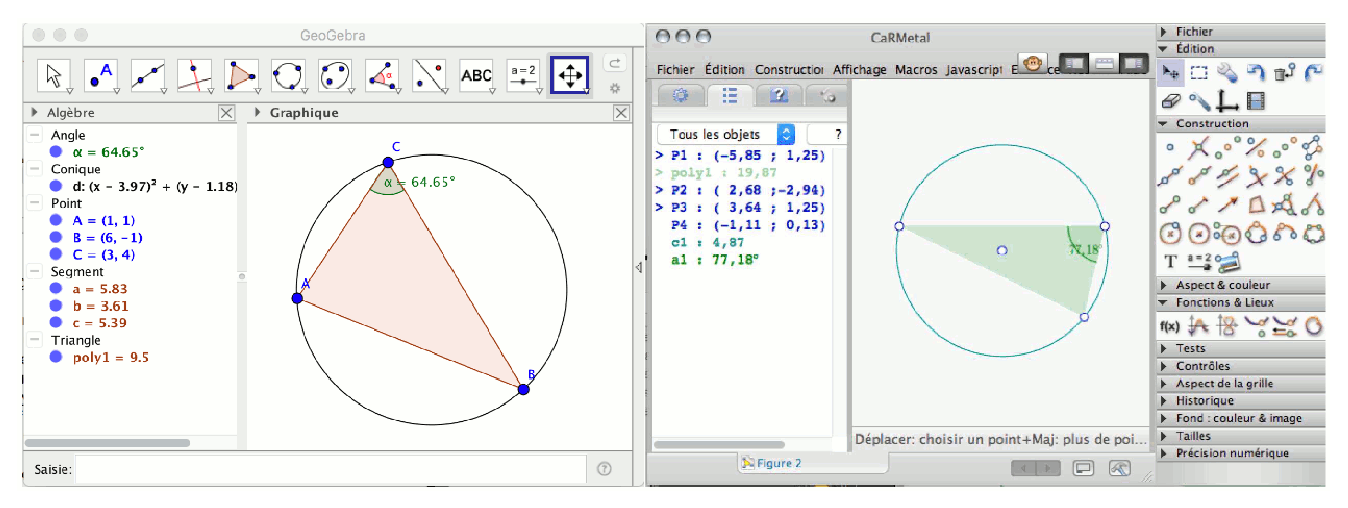
\includegraphics[height=6.1cm]{Geometrie/Images/G9_cours_dynamique} \\
   GeoGebra \hspace{7cm} CaRMetal
\end{center}


\section{Propriétés} %%%

Ci-dessous une série de propriétés géométriques issues du \href{http://mep-outils.sesamath.net/manuel_numerique/index.php?ouvrage=ms2_2014&page_gauche=267}{\blue manuel Sesamath} de seconde.

{\renewcommand{\StringDOCUMENTATION}{Une trame pour démontrer en géométrie}
\begin{documentation}
\begin{itemize}
   \item Commencer par réaliser un {\bf schéma} représentant la situation de l'énoncé ;
   \item penser à {\bf coder} les milieux, les angles droits et à repasser en couleurs les droites ou segments parallèles donnés par l'énoncé ;
   \item parmi les propriétés qui correspondent à la question posée, {\bf choisir} celle dont la figure de la première colonne s'apparente le mieux à celle du schéma réalisé. \\ [-8mm]
\end{itemize}
\end{documentation}}

\bigskip

\subsection{Démontrer qu'un point est le milieu d'un segment}%A%


{\small
\begin{tableau}[pr]{\linewidth}
   \hline %%%%%%%%%%%%%%%%%%%%%%P1 
   \begin{tikzpicture}[scale=0.5]
      \draw(0,0)--(4,2);
      \draw (1,0.5) node[color=A1,rotate=-60]{$\approx$};
      \draw (3,1.5) node[color=A1,rotate=-60]{$\approx$};
      \draw (0,0) node{$\times$};
      \draw (4,2) node{$\times$};
      \draw (2,1) node{$\times$};
      \draw (0,0) node[left]{$A$};
      \draw (4,2) node[right]{$B$};
      \draw (2,1) node[above]{$O$};
   \end{tikzpicture}
   &
   \propriete{} Si un point, sur un segment, est à égale distance des deux extrémités, alors ce point est le milieu du segment. \newline
   &
   Ici, $O\in [AB]$ et $OA=OB$. \newline  
   Donc $O$ est le milieu de $[AB]$. \\
   \hline %%%%%%%%%%%%%%%%%%%%%%P2
   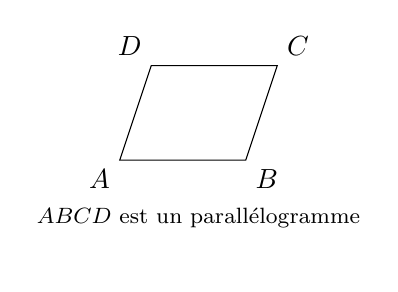
\begin{tikzpicture}[scale=0.4] 
      \draw (0,0)--(4,0)--(5,3)--(1,3)--cycle;
      \draw (0,0) node[below left] {$A$};
      \draw (4,0) node[below right] {$B$};
      \draw (5,3) node[above right] {$C$};
      \draw (1,3) node[above left] {$D$};
      \draw (2.5,-1.2) node[below] {\footnotesize $ABCD$ est un parallélogramme};
      \draw (0,-3) node {};
   \end{tikzpicture}
   &
   \propriete{} Si un quadrilatère est un parallélogramme alors ses diagonales se coupent en leur milieu (c'est aussi vrai pour les losanges, rectangles et carrés qui sont des parallélogrammes particuliers).
   &
   Ici, $ABCD$ est un parallélogramme. \newline
   Donc ses diagonales $[AC]$ et $[BD]$ se coupent en leur milieu. \\    
   \hline %%%%%%%%%%%%%%%%%%%%%%P3
   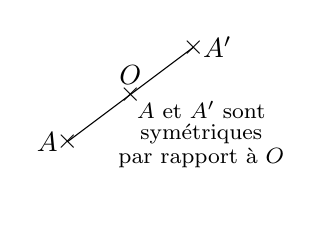
\begin{tikzpicture}[scale=0.4]
      \draw(0,0)--(4,3);
      \draw (0,0) node{$\times$};
      \draw (4,3) node{$\times$};
      \draw (2,1.5) node{$\times$};
      \draw (0,0) node[left]{$A$};
      \draw (4,3) node[right]{$A'$};
      \draw (2,1.5) node[above]{$O$};
      \draw (4.25,1) node{\footnotesize $A$ et $A'$ sont};
      \draw (4.25,0.25) node{\footnotesize symétriques};
      \draw (4.25,-0.5) node{\footnotesize par rapport à $O$};
      \draw (0,-1.5) node {};
   \end{tikzpicture}
   &
   \propriete{} Si deux points sont symétriques par rapport à un point alors le centre de symétrie est le milieu du segment d'extrémités les deux symétriques.
   & 
   Ici, $A$ et $A'$ sont symétriques par rapport au point $O$. \newline  
   Donc $O$ est le milieu du segment $[AA']$. \\
   \hline %%%%%%%%%%%%%%%%%%%%%%P4
   \begin{tikzpicture}[scale=0.5]
      \draw (0.5,2.825)--(3.5,2.125);
      \draw[very thick, color=B2] (1.5,0.5)--(2.5,4.5);
      \foreach \x/\y/\N/\pos in {0.5/2.825/A/left, 3.5/2.125/B/right} {\draw (\x,\y) node{$\times$};\draw (\x,\y) node[\pos]{$\N$}; } 
      \draw (2,2.5) node[below left] {$O$};
      \draw (3,4) node {$(d)$};
      \draw (2.5,0) node{\footnotesize $(d)$ est la médiatrice de $[AB]$};
      \draw (1,-0.7) node {};
   \end{tikzpicture}
   &
   \propriete{} Si une droite est la médiatrice d'un segment alors elle coupe ce segment en son milieu.
   &
   Ici, la médiatrice de $[AB]$ coupe $[AB]$ en $O$. \newline
   Donc $O$ est le milieu de $[AB]$. \\
   \hline %%%%%%%%%%%%%%%%%%%%%%P5
   \begin{tikzpicture}[ scale=0.4]
      \draw (0,0)--(5,1)--(1,4)--cycle;
      \draw[very thick, color=B2] (-1,1.75)--(4,2.75);
      \draw[very thick, color=B2] (0,0)--(5,1);
      \foreach \x/\y/\N/\pos in {0/0/A/left, 5/1/B/right, 1/4/C/above left, 0.5/2/I/above left, 3/2.5/J/above right} {%\draw (\x,\y) node{$\times$};
      \draw (\x,\y) node[\pos]{$\N$}; } 
      \draw (0.25,1) node[rotate=7, color=A1] {$\approx$};
      \draw (0.75,3) node[rotate=7, color=A1] {$\approx$};
      \draw (0,-1) node {};
   \end{tikzpicture}
   &
   \propriete{} Si, dans un triangle, une droite passe par le milieu d'un côté et est parallèle à un deuxième côté alors elle passe par le milieu du troisième côté.
   &
   Ici, dans le triangle $ABC$, $I$ est le milieu de $[AC]$ et la parallèle à $[AB]$ passant par $I$ coupe $[BC]$ en $J$. Donc $J$ est le milieu du segment $[BC]$. \newline \\ 
   \hline 
\end{tableau}}
 

 \subsection{Démontrer que deux droites sont parallèles}%B%
 %%%%%%%%%%%%%%%%%%%%%%%%%%%%%
 
\begin{tableau}[pr]{\linewidth}
   \hline %%%%%%%%%%%%%%%%%%%%%%P6
   \begin{tikzpicture}[scale=0.5]
      \draw[very thick,color=A2] (0,0)--(3,2);
      \draw[very thick,color=A2] (1,0)--(4,2);
      \draw[very thick, color=B2, loosely dashed] (1,0)--(4,2);
      \draw[very thick, color=B2] (4,0)--(7,2);
      \draw (3,2) node[above left] {$(d_1)$};
      \draw (4,2) node[above] {$(d_2)$};
      \draw (4,0) node[below right] {$(d_3)$};
      \draw (4,-1.5) node{};
   \end{tikzpicture}
   &
   \propriete{}  Si deux droites sont parallèles alors toute droite parallèle à l'une est parallèle à l'autre.
   &
   Ici,  $(d_1)//(d_2)$ et $(d_2)//(d_3)$.  Donc   $(d_1)//(d_3)$. \\ [-3mm]
   \hline %%%%%%%%%%%%%%%%%%%%%%P7
   \begin{tikzpicture}[ scale=0.5]
      \draw[fill=G1, shift={(2.05,1.5)}, rotate=14] (0,0) rectangle (0.25,0.25);
      \draw[fill=G1, shift={(2.25,0.55)}, rotate=14] (0,0) rectangle (0.25,0.25);
      \draw (0,0)--(4,1);
      \draw (0,1)--(4,2);
      \draw[color=B2, very thick] (1.75,2.75)--(2.5,-0.5);
      \draw (4,2) node[above right] {$(d_1)$};
      \draw (4,1) node[right] {$(d_2)$};
      \draw (1.75,2.75) node[above left] {$(d_3)$};
      \draw (4,-1) node{};
   \end{tikzpicture}
   &
   \propriete{} Si deux droites sont perpendiculaires à la même droite alors elles sont parallèles entre elles.
   &
   Ici,  $(d_1)\perp(d_3)$ et $(d_2)\perp(d_3)$.  Donc $(d_1)//(d_2)$. \\ [-3mm]
   \hline %%%%%%%%%%%%%%%%%%%%%%P8
   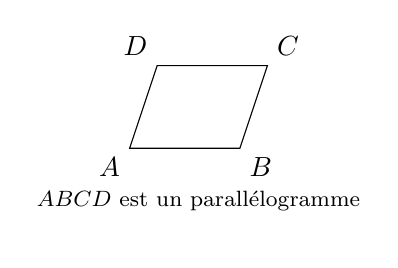
\begin{tikzpicture}[scale=0.35] 
      \draw (0,0)--(4,0)--(5,3)--(1,3)--cycle;
      \draw (0,0) node[below left] {$A$};
      \draw (4,0) node[below right] {$B$};
      \draw (5,3) node[above right] {$C$};
      \draw (1,3) node[above left] {$D$};
      \draw (2.5,-1.2) node[below] {\footnotesize $ABCD$ est un parallélogramme};
      \draw (2,-3) node {};
   \end{tikzpicture}
   &
   \propriete{} Si un quadrilatère est un parallélogramme alors ses côtés opposés sont parallèles.
   &
   Ici, $ABCD$ est un parallélogramme. \newline
   Donc $(AB)//(DC)$ et $(AD)//(BC)$. \\ [-3mm]
   \hline %%%%%%%%%%%%%%%%%%%%%%P8
   \begin{tikzpicture}[ scale=0.45]
      \draw (0,0)--(5,1)--(1,4)--cycle;
      \draw (-1,1.75)--(4,2.75);
      \draw (0,0)--(5,1);
      \foreach \x/\y/\N/\pos in {0/0/A/left, 5/1/B/right, 1/4/C/above left, 0.5/2/I/above left, 3/2.5/J/above right} {%\draw (\x,\y) node{$\times$};
      \draw (\x,\y) node[\pos]{$\N$}; } 
      \draw (0.25,1) node[rotate=7, color=A1] {$\approx$};
      \draw (0.75,3) node[rotate=7, color=A1] {$\approx$};
      \draw (2,3.25) node[color=C1] {$\circ$};
      \draw (4,1.75) node[color=C1] {$\circ$};
      \draw (2,-1) node {};
   \end{tikzpicture}
   &
   \propriete{} Si, dans un triangle, une droite passe par les milieux de deux côtés alors elle est parallèle au troisième côté.
   &
   Ici, dans le triangle $ABC$, $I$ est le milieu de $[AC]$ et $J$ est le milieu de $[BC]$. \newline
   Donc $(IJ)$ est parallèle à $(AB)$. \\ [-3mm]
   \hline %%%%%%%%%%%%%%%%%%%%%%P10
   \begin{tikzpicture}[ xscale=0.45, yscale=0.8]
      \draw (0,0)--(6,0);
      \draw (0,2)--(6,2);
      \draw (0,-0.75)--(5,3.25);
      \draw (0,2.5)--(6,-0.5);
      \draw (2.5,1.25) node[right] {$A$};
      \draw (5,0) node[below left] {$B$};
      \draw (0.75,0) node[below right] {$C$};
      \draw (1,2) node[above] {$M$};
      \draw (3.25,2) node[above] {$N$};
      \draw (2,-1.2) node {};
      \draw (6,1) node {\footnotesize $\dfrac{AM}{AB}=\dfrac{AN}{AC}$} ;
   \end{tikzpicture}
   &
   \propriete{}
   Si les points $B$, $A$, $M$ d'une part et les points $C$, $A$, $N$ d'autre part sont alignés dans le même ordre et si $\dfrac{AB}{AM}=\dfrac{AC}{AN}$ alors les droites $(CB)$ et $(MN)$ sont parallèles.
   &
   $M$, $A$, $B$ d'une part et $N$, $A$, $C$ d'autre part sont alignés dans cet ordre. De plus, $\dfrac{AM}{AB}=\dfrac{AN}{AC}$. \newline
   Donc $(MN)//(CB)$. \\  [-3mm]
   \hline %%%%%%%%%%%%%%%%%%%%%%P11
   \begin{tikzpicture}[ scale=0.6]
      \draw (0,0)--(4,2);
      \draw (0,2)--(4,4);
      \draw[dashed] (0.5,0.25)--(3.5,3.75);
      \draw[dashed] (1,2.5)--(3,1.5);
      \foreach \x/\y/\N/\pos in {0.5/0.25/A/below left, 3.5/3.75/B/above, 1/2.5/C/above left, 3/1.5/D/below right,2/2/O/below} {\draw (\x,\y) node{$\times$};
      \draw (\x,\y) node[\pos]{$\N$}; } 
      \draw (1.25,1.125) node[rotate=-20, color=A1] {$\approx$};
      \draw (2.75,2.825) node[rotate=-20, color=A1] {$\approx$};
      \draw (1.5,2.25) node[color=C1] {$\circ$};
      \draw (2.5,1.75) node[color=C1] {$\circ$};
      \draw (2,-0.8) node {};
   \end{tikzpicture}
   &
   \propriete{} Si deux droites sont symétriques par rapport à un point alors elles sont parallèles.
   &
   Ici, $(AD)$ et $(BC)$ sont symétriques par rapport à $O$. \newline
   Donc $(AD)//(CB)$. \\
   \hline
\end{tableau}
 

\subsection{Démontrer que deux droites sont perpendiculaires}%C%

 
\begin{tableau}[pr]{\linewidth}
   \hline %%%%%%%%%%%%%%%%%%%%%%P12
   \begin{tikzpicture}[ scale=0.65]
      \draw[shift={(2.05,1.5)}, rotate=14, fill=G1] (0,0)rectangle(0.3,0.3);
      \draw[color=B2, very thick] (0,0)--(4,1);
      \draw[color=B2, very thick] (0,1)--(4,2);
      \draw (1.75,2.75)--(2.5,-0.5);
      \draw (4,2) node[above right] {$(d_1)$};
      \draw (4,1) node[right] {$(d_2)$};
      \draw (1.75,2.75) node[left] {$(d_3)$};
      \draw (0,-1) node {};
   \end{tikzpicture}
   &
   \propriete{} 
   Si deux droites sont parallèles alors toute droite perpendiculaire à l'une est perpendiculaire à l'autre.
   &
   Ici, $(d_1)//(d_2)$ et $(d_1)\perp(d_3)$ \newline
    Donc  $(d_2)\perp(d_3)$. \\ [-4mm]
    \hline %%%%%%%%%%%%%%%%%%%%%%P13
    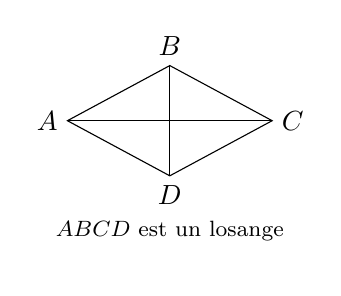
\begin{tikzpicture}[ xscale=0.65, yscale=0.7]
       \draw (0,0)--(2,-1)--(4,0)--(2,1)--cycle;
       \draw (0,0)--(4,0);
       \draw (2,-1)--(2,1);
       \draw (0,0) node[left] {$A$};
       \draw (2,1) node[above] {$B$};
       \draw (4,0) node[right] {$C$};
       \draw (2,-1) node[below] {$D$};
       \draw (2,-2) node{\footnotesize $ABCD$ est un losange};
       \draw (0,-2.5) node {};
    \end{tikzpicture}
    &
    \propriete{} Si un quadrilatère est un losange alors ses diagonales sont perpendiculaires (c'est aussi vrai pour le carré qui est un losange particulier). 
    &
    Ici, $ABCD$ est un losange. \newline
    Donc $(AC)\perp(BD)$. \\ [-4mm]
    \hline %%%%%%%%%%%%%%%%%%%%%%P14
    \begin{tikzpicture}[ scale=0.6]
       \draw (0.5,2.825)--(3.5,2.125);
       \draw[very thick, color=B2] (1.5,0.5)--(2.5,4.5);
       \foreach \x/\y/\N/\pos in {0.5/2.825/A/left, 3.5/2.125/B/right} {\draw (\x,\y) node{$\times$};\draw (\x,\y) node[\pos]{$\N$}; } 
       \draw (2,2.5) node[below left] {$O$};
       \draw (3,4) node {$(d)$};
       \draw (2.5,0) node{\footnotesize $(d)$ est la médiatrice de $[AB]$};
       \draw (0,-0.8) node {};
    \end{tikzpicture}
    &
    \propriete{} Si une droite est la médiatrice d'un segment alors elle est perpendiculaire à ce segment.
    &
    Ici, $(d)$ est la médiatrice du segment $[AB]$. \newline
    Donc $(d)\perp(AB)$. \\ [-4mm]
    \hline %%%%%%%%%%%%%%%%%%%%%%P15
   \begin{tikzpicture}[scale=1.06]
      \draw (0,0) circle (1);
      \draw (0,0) node{$\times$};
      \draw (0,-1.414) node[left]{$(d)$};
      \draw (1,1) node{$(\mathscr C)$};
      \draw (0.71,-0.71) node[below right]{$T$};
      \draw (0,0) node[below left]{$O$};
      \draw[very thick, color=B2] (0,-1.414)--(2,0.586);
      \draw[dashed, color=B2] (0,0)--(0.71,-0.71);
      \draw (0,-1.8) node {};
   \end{tikzpicture}
   &
   \propriete{} Si une droite est tangente à un cercle en un point alors elle est perpendiculaire au rayon de ce cercle qui a pour extrémité ce point.
   &
   Ici, la droite $(d)$ est la tangente en $T$ au cercle de centre $O$. \newline
   Donc $(d)\perp(OT)$. \\ [-4mm]
   \hline %%%%%%%%%%%%%%%%%%%%%%P26
   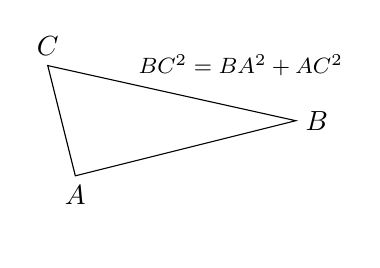
\begin{tikzpicture}[ scale=0.7]
      \draw (0,0)--(4,1)--(-0.5,2)--cycle;
      \draw (0,0) node[below] {$A$};
      \draw (4,1) node[right] {$B$};
      \draw (-0.5,2) node[above] {$C$};
      \draw (3,2) node {\footnotesize $BC^2=BA^2+AC^2$};
      \draw (0,-1) node {};
   \end{tikzpicture} &
   \propriete{}
   Si, dans un triangle, le carré de la longueur du plus grand côté est égal à la somme des carrés des longueurs des deux autres côtés alors le triangle est rectangle. \newline
   &
   Ici, $BC^2=BA^2+AC^2$. \newline
   Donc, le triangle $ABC$ est rectangle en $A$. \\ [-4mm]
   \hline %%%%%%%%%%%%%%%%%%%%%%P17
   \begin{tikzpicture}[ scale=1.4]
      \draw (0,0) circle (1);
      \draw (-0.953,-0.3)--(0.953,0.3)--(-0.5,0.87)--cycle;
      \draw (0,0) node {$\times$};
      \draw (0.477,0.15) node[color=A1, rotate=107.45] {$\approx$};
      \draw (-0.477,-0.15) node[color=A1, rotate=107.45] {$\approx$};
     \draw (-0.953,-0.3) node[left] {$A$};
     \draw (0.953,0.3) node[right] {$B$};
     \draw (-0.5,0.87) node[above] {$C$};
     \draw (0,-1.3) node {};
   \end{tikzpicture}
   &
   \propriete{} Si un triangle est inscrit dans un cercle de diamètre l'un de ses côtés alors il est rectangle et il admet ce diamètre pour hypoténuse.
   &
   Ici, $C$ appartient au cercle de diamètre $[AB]$. \newline
   Donc $ABC$ est rectangle en $C$. \\
   \hline 
\end{tableau}
 


\subsection{Démontrer qu'un quadrilatère est un parallélogramme}%D%

 
\begin{tableau}[pr]{\linewidth}
   \hline %%%%%%%%%%%%%%%%%%%%%%P18
   \begin{tikzpicture}[xscale=0.5,yscale=0.2]
      \draw[color=A1, very thick] (0,0)--(4,1);
      \draw[color=A1, very thick] (1,4)--(5,5);
      \draw[color=B2, very thick] (0,0)--(1,4);
      \draw[color=B2, very thick] (4,1)--(5,5);
      \draw (0,0) node[below left] {$A$};
      \draw (4,1) node[below right] {$B$};
      \draw (5,5) node[above right] {$C$};
      \draw (1,4) node[above] {$D$};
      \draw (0,-2.3) node {};
   \end{tikzpicture}
   &
   \propriete{} Si un quadrilatère a ses côtés opposés parallèles deux à deux alors c'est un parallélogramme. 
   &
   Ici, $(AB)//(DC)$ et $(AD)//(BC)$.  \newline
   Donc $ABCD$ est un parallélogramme. \\ [-5mm]
   \hline %%%%%%%%%%%%%%%%%%%%%%P19
   \begin{tikzpicture}[ xscale=0.5,yscale=0.5]
      \draw (0,0)--(4,1)--(5,3)--(1,2)--cycle;
      \draw (0,0)--(5,3);
      \draw (4,1)--(1,2);
      \draw (0,0) node[below left]{$A$};
      \draw (4,1) node[below right]{$B$};
      \draw (4.7,3) node[above right]{$C$};
      \draw (1,2) node[above left]{$D$};
      \draw (1.25,0.75) node[color=A1,rotate=120.96] {$\approx$};
      \draw (1.75,1.75) node[color=C1,rotate=-120.96] {$\circ$};
      \draw (3.75,2.25) node[color=A1,rotate=120.96] {$\approx$};
      \draw (3.25,1.25) node[color=C1,rotate=-120.96] {$\circ$};
      \draw (0,-1) node {};
   \end{tikzpicture}
   &
   \propriete{} Si un quadrilatère a ses diagonales qui se coupent en leur milieu alors c'est un parallélogramme.    
   & Ici, $[AC]$ et $[BD]$ se coupent en leur milieu. \newline
   Donc, $ABCD$ est un parallélogramme. \\ [-5mm]
   \hline %%%%%%%%%%%%%%%%%%%%%%P20
   \begin{tikzpicture}[ scale=0.5]
      \draw (0,0)--(4,1)--(5,3)--(1,2)--cycle;
      \draw[very thick, color=B2] (0,0)--(4,1);
      \draw[very thick, color=B2] (5,3)--(1,2);
      \draw (0,0) node[below left]{$A$};
      \draw (4,1) node[below right]{$B$};
      \draw (5,3) node[above right]{$C$};
      \draw (1,2) node[above left]{$D$};
      \draw (2,0.5) node[color=A1,rotate=104] {$\approx$};
      \draw (3,2.5) node[color=A1,rotate=104] {$\approx$};
      \draw (0,-0.8) node {};
   \end{tikzpicture}
   &
   \propriete{} Si un quadrilatère non croisé a deux côtés opposés parallèles de même longueur alors c'est un parallélogramme.
   &
   Ici, $ABCD$ est non croisé avec $AB=DC$ et $(AB)//(CD)$. \newline
   Donc, $ABCD$ est un parallélogramme. \\ [-5mm]
   \hline %%%%%%%%%%%%%%%%%%%%%%P21
   \begin{tikzpicture}[ scale=0.5]
      \draw (0,0)--(4,1)--(5,3)--(1,2)--cycle;
      \draw (0,0) node[left]{$A$};
      \draw (4,1) node[below right]{$B$};
      \draw (5,3) node[above right]{$C$};
      \draw (1,2) node[above left]{$D$};
      \draw (2,0.5) node[color=A1,rotate=104] {$\approx$};
      \draw (0.5,1) node[color=C1,rotate=153.43] {$\circ$};
      \draw (3,2.5) node[color=A1,rotate=104] {$\approx$};
      \draw (4.5,2) node[color=C1,rotate=153.43] {$\circ$};
      \draw (0,-0.4) node {};
   \end{tikzpicture}
   &
   \propriete{} Si un quadrilatère a ses côtés opposés de la même longueur deux à deux alors c'est un parallélogramme.
   & Ici, $AB=DC$ et $AD=BC$. \newline
   Donc, $ABCD$ est un parallélogramme. \\
   \hline
\end{tableau}


\subsection{Démontrer qu'un quadrilatère est un losange}%E%


\begin{tableau}[pr]{\linewidth}
   \hline %%%%%%%%%%%%%%%%%%%%%%P22
   \begin{tikzpicture}[ xscale=0.7, yscale=0.5]
      \draw (0,-1)--(2,0)--(0,1)--(-2,0)--cycle;
      \draw (0,-1) node[below] {$A$};
      \draw (2,0) node[right] {$B$};
      \draw (0,1) node[above] {$C$};
      \draw (-2,0) node[left] {$D$};
      \draw (1,0.5) node[color=A1, rotate=63.435] {$\approx$};
      \draw (-1,0.5) node[color=A1, rotate=116.565] {$\approx$};
      \draw (1,-0.5) node[color=A1, rotate=116.565] {$\approx$};
      \draw (-1,-0.5) node[color=A1, rotate=63.435] {$\approx$};
      \draw (0,-2) node {};
   \end{tikzpicture}
   &
   \propriete{} Si un quadrilatère a ses quatre côtés de même longueur alors c'est un losange.
   &
   Ici, $AB=BC=CD=DA$. \newline
   Donc $ABCD$ est un losange. \\ [-5mm]
   \hline %%%%%%%%%%%%%%%%%%%%%%P23
   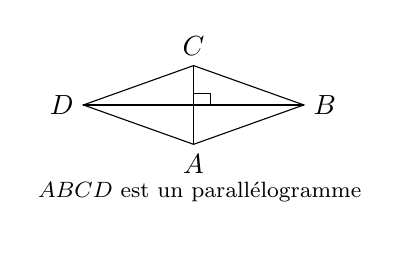
\begin{tikzpicture}[ xscale=0.7, yscale=0.5]
      \draw (0,-1)--(2,0)--(0,1)--(-2,0)--cycle;
      \draw (0,-1) node[below] {$A$};
      \draw (2,0) node[right] {$B$};
      \draw (0,1) node[above] {$C$};
      \draw (-2,0) node[left] {$D$};
      \draw (0,0) rectangle (0.3,0.3);
      \draw (2,0)--(-2,0);
      \draw (0,-1)--(0,1);
      \draw (-3,-2.2) node[right]{\footnotesize $ABCD$ est un parallélogramme};
      \draw (0,-2.8) node {};
   \end{tikzpicture}
   &
   \propriete{} Si un parallélogramme a ses diagonales perpendiculaires alors c'est un losange.
   &
   Ici, $ABCD$ est un parallélogramme et $(AC)\perp(BD)$. \newline
   Donc $ABCD$ est un losange. \\ [-5mm]
   \hline %%%%%%%%%%%%%%%%%%%%%%P24
   \begin{tikzpicture}[ xscale=0.7, yscale=0.5]
      \draw (0,-1)--(2,0)--(0,1)--(-2,0)--cycle;
      \draw (0,-1) node[below] {$A$};
      \draw (2,0) node[right] {$B$};
      \draw (0,1) node[above] {$C$};
      \draw (-2,0) node[left] {$D$};
      \draw (1,0.5) node[color=A1, rotate=63.435] {$\approx$};
      \draw (-1,0.5) node[color=A1, rotate=116.565] {$\approx$};
      \draw (-3,-2.2) node[right]{\footnotesize $ABCD$ est un parallélogramme};
      \draw (0,-2.8) node {};
   \end{tikzpicture}
   &
   \propriete{} Si un parallélogramme a deux côtés consécutifs de la même longueur alors c'est un losange.
   &
   Ici, $ABCD$ est un parallélogramme avec $CD=CB$. \newline
   Donc $ABCD$ est un losange. \\
   \hline 
\end{tableau}


\subsection{Démontrer qu'un quadrilatère est un rectangle}%F%


\begin{tableau}[pr]{\linewidth}
   \hline %%%%%%%%%%%%%%%%%%%%%%P25
   \begin{tikzpicture}[ scale=0.58]
      \draw (0,0)--(3,0)--(3,2)--(0,2)--cycle;
      \draw (0,0) node[left]{$A$};
      \draw (3,0) node[right]{$B$};
      \draw (3,2) node[right]{$C$};
      \draw (0,2) node[left]{$D$};
      \draw (0,0) [fill=G1] rectangle (0.3,0.3);
      \draw (3,0) [fill=G1] rectangle (2.7,0.3);
      \draw (3,2) [fill=G1] rectangle (2.7,1.7);
      \draw (0,-0.8) node {};
   \end{tikzpicture}
   &
   \propriete{} Si un quadrilatère possède trois angles droits alors c'est un rectangle.
   &
   Ici, $(AD)\perp(AB)$, $(AB)\perp(BC)$ et $(BC)\perp(DC)$. \newline
   Donc $ABCD$ est un rectangle. \\ [-4mm]
   \hline %%%%%%%%%%%%%%%%%%%%%%P26
   \begin{tikzpicture}[ scale=0.58]
      \draw (0,0)--(3,0)--(3,2)--(0,2)--cycle;
      \draw (0,0) node[left]{$A$};
      \draw (3,0) node[right]{$B$};
      \draw (3,2) node[right]{$C$};
      \draw (0,2) node[left]{$D$};
      \draw (1.5,-1.1) node{\footnotesize $ABCD$ est un parallélogramme};
      \draw (0,0)--(3,2); 
      \draw (0,2)--(3,0);
      \draw (0.75,0.5) node[color=A1, rotate=123.69] {$\approx$};
      \draw (2.25,0.5) node[color=A1, rotate=56.31] {$\approx$};
      \draw (0.75,1.5) node[color=A1, rotate=56.31] {$\approx$};
      \draw (2.25,1.5) node[color=A1, rotate=123.69] {$\approx$};
      \draw (0,-1.7) node {};
   \end{tikzpicture}
   &
   \propriete{} Si un parallélogramme a ses diagonales de la même longueur alors c'est un rectangle.
   &
   Ici, $ABCD$ est un parallélogramme avec $AC=BD$. \newline
   Donc $ABCD$ est un rectangle. \\ [-4mm]
   \hline %%%%%%%%%%%%%%%%%%%%%%P27
   \begin{tikzpicture}[ scale=0.58]
      \draw (0,0)--(3,0)--(3,2)--(0,2)--cycle;
      \draw (0,0) node[left]{$A$};
      \draw (3,0) node[right]{$B$};
      \draw (3,2) node[right]{$C$};
      \draw (0,2) node[left]{$D$};
      \draw (3,2) [fill=G1] rectangle (2.7,1.7);
      \draw (1.5,-1.1) node{\footnotesize $ABCD$ est un parallélogramme};
      \draw (0,-1.7) node {};
   \end{tikzpicture}
   &
   \propriete{} Si un parallélogramme possède deux côtés consécutifs perpendiculaires alors c'est un rectangle.
   &
   Ici, $ABCD$ est un parallélogramme avec $(BC)\perp(CD)$. \newline
   Donc $ABCD$ est un rectangle. \\
   \hline 
\end{tableau}


\subsection{Démontrer qu'un quadrilatère est un carré}%G%


\begin{tableau}[pr]{\linewidth}
   \hline%%%%%%%%%%%%%%%%%%%%%%P28
   \begin{tikzpicture}[ scale=0.6]
      \draw (0,0)--(2,0)--(2,2)--(0,2)--cycle;
      \draw (0,0) node[left]{$A$};
      \draw (2,0) node[right]{$B$};
      \draw (2,2) node[right]{$C$};
      \draw (0,2) node[left]{$D$};
      \draw (1,-0.6) node{\footnotesize $ABCD$ est un rectangle};
      \draw (1,0) node[color=A1, rotate=90]{$\approx$};
      \draw (0,1) node[color=A1]{$\approx$};
      \draw (0,-1) node {};
   \end{tikzpicture}
   &
   \propriete{}Si un rectangle possède deux côtés consécutifs de même longueur alors c'est un carré.
   &
   Ici, $ABCD$ est un rectangle avec $AB=AD$. \newline
    Donc $ABCD$ est un carré. \\ [-4mm]
    \hline %%%%%%%%%%%%%%%%%%%%%%P29
    \begin{tikzpicture}[ scale=0.6]
       \draw (0,0)--(2,0)--(2,2)--(0,2)--cycle;
       \draw (0,0) node[left]{$A$};
       \draw (2,0) node[right]{$B$};
       \draw (2,2) node[right]{$C$};
       \draw (0,2) node[left]{$D$};
       \draw (0,0) [fill=G1] rectangle (0.3,0.3);
       \draw (1,-0.6) node{\footnotesize $ABCD$ est un losange};
       \draw (0,-1) node {};
   \end{tikzpicture}
   &
   \propriete{}
   Si un losange possède deux côtés consécutifs perpendiculaires alors c'est un carré.
   &
   Ici, $ABCD$ est un losange avec $(AB)\perp(AD)$. \newline
   Donc $ABCD$ est un carré. \\ [-4mm]
   \hline %%%%%%%%%%%%%%%%%%%%%%P30 
   \begin{tikzpicture}[ scale=0.6]
      \draw (0,0)--(2,0)--(2,2)--(0,2)--cycle;
      \draw (0,0) node[left]{$A$};
      \draw (2,0) node[right]{$B$};
      \draw (2,2) node[right]{$C$};
      \draw (0,2) node[left]{$D$};
      \draw (0,0)--(2,2);
      \draw (0,2)--(2,0);
      \draw [shift={(1,1)}, rotate=45,fill=G1] (0,0) rectangle (0.3,0.3);
      \draw (1,-0.6) node{\footnotesize $ABCD$ est un rectangle};
      \draw (0,-1) node {};
   \end{tikzpicture}
   &
   \propriete{} Si un  rectangle a ses diagonales perpendiculaires alors c'est un carré.
   &
   Ici, $ABCD$ est un rectangle avec $(AC)\perp(BD)$. \newline
   Donc $ABCD$ est un carré. \\ [-4mm]
   \hline %%%%%%%%%%%%%%%%%%%%%%P31
   \begin{tikzpicture}[ scale=0.6]
      \draw (0,0)--(2,0)--(2,2)--(0,2)--cycle;
      \draw (0,0) node[left]{$A$};
      \draw (2,0) node[right]{$B$};
      \draw (2,2) node[right]{$C$};
      \draw (0,2) node[left]{$D$};
      \draw (0,0)--(2,2);
      \draw (0,2)--(2,0);
      \draw (0.5,0.5) node[color=A1, rotate=-45]{$\approx$};
      \draw (1.5,0.5) node[color=A1, rotate=45]{$\approx$};
      \draw (0.5,1.5) node[color=A1, rotate=45]{$\approx$};
      \draw (1.5,1.5) node[color=A1, rotate=-45]{$\approx$};
      \draw (1,-0.6) node{\footnotesize $ABCD$ est un losange};
      \draw (0,-1) node {};
   \end{tikzpicture}
   & 
   \propriete{} Si un  losange a ses diagonales de même longueur alors c'est un carré.
   &
   Ici, $ABCD$ est un losange avec $AC=BD$. \newline
   Donc $ABCD$ est un carré. \\
   \hline 
\end{tableau}


\subsection{Déterminer la mesure d'un segment} %H%

 
\begin{tableau}[pr]{\linewidth}
  \hline %%%%%%%%%%%%%%%%%%%%%%P32
   \begin{tikzpicture}[ yscale=0.6]
      \draw (0,0)--(2,0)--(1,2)--cycle;
      \draw (0,0) node[left]{$A$};
      \draw (2,0) node[right]{$B$};
      \draw (1,2) node[right]{$C$};
      \draw (0.5,1) node[rotate=-26.56, color=B2]{$\approx$};
      \draw (1.5,1) node[rotate=26.56, color=B2]{$\approx$};
      \draw (0,-0.5) node {};
   \end{tikzpicture}
   &
   \propriete{} Si un triangle est isocèle [resp. équilatéral] alors il a deux [resp. trois] côtés de même longueur.
   &
   Ici, $ABC$ est isocèle en $C$. \newline
   Donc $CA=CB$. \\ [-4mm]
   \hline %%%%%%%%%%%%%%%%%%%%%%P33
   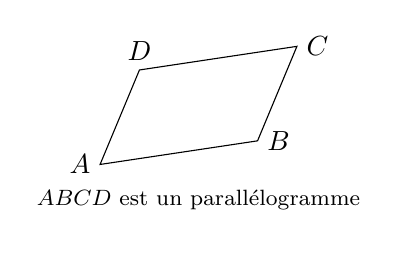
\begin{tikzpicture}[ xscale=0.5, yscale=0.3]
      \draw (0,0)--(4,1)--(5,5)--(1,4)--cycle;
      \draw (0,0) node[left] {$A$};
      \draw (4,1) node[right] {$B$};
      \draw (5,5) node[right] {$C$};
      \draw (1,4) node[above] {$D$};
      \draw (2.5,-1.5) node{\footnotesize $ABCD$ est un parallélogramme};
      \draw (0,-2.5) node {};
   \end{tikzpicture}
   &
   \propriete{} Si un quadrilatère est un parallélogramme alors ses côtés opposés ont la même longueur (c'est également vrai pour les rectangles, les losanges et les carrés qui sont des parallélogrammes particuliers).
   &
   Ici, $ABCD$ est un parallélogramme. \newline
   Donc $AB=DC$ et $AD=BC$. \\ [-4mm]
   \hline %%%%%%%%%%%%%%%%%%%%%%P34
   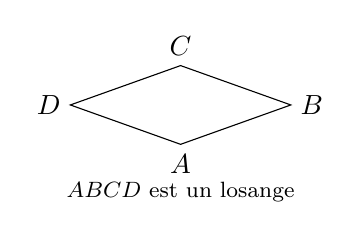
\begin{tikzpicture}[ xscale=0.7, yscale=0.5]
      \draw (0,-1)--(2,0)--(0,1)--(-2,0)--cycle;
      \draw (0,-1) node[below] {$A$};
      \draw (2,0) node[right] {$B$};
      \draw (0,1) node[above] {$C$};
      \draw (-2,0) node[left] {$D$};
      \draw (0,-2.2) node{\footnotesize $ABCD$ est un losange};
      \draw (0,-2.7) node {};
   \end{tikzpicture}
   &
   \propriete{} Si un quadrilatère est un losange alors tous ses côtés sont de la même longueur (c'est également vrai pour les carrés qui sont des losanges particuliers).
   &
   Ici, $ABCD$ est un losange. \newline
   Donc $AB=BC=CD=DA$. \\ [-4mm]
   \hline %%%%%%%%%%%%%%%%%%%%%%P35
   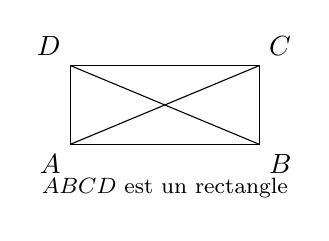
\begin{tikzpicture}[ xscale=0.8, yscale=0.5]
      \draw (0,0)--(3,0)--(3,2)--(0,2)--cycle;
      \draw (0,0) node[below left] {$A$};
      \draw (3,0) node[below right] {$B$};
      \draw (3,2) node[above right] {$C$};
      \draw (0,2) node[above left] {$D$};
      \draw (0,0)--(3,2);
      \draw (0,2)--(3,0);
      \draw (1.5,-0.6) node[below]{\footnotesize $ABCD$ est un rectangle};
      \draw (0,-1.5) node {};
   \end{tikzpicture}
   &
   \propriete{} Si un quadrilatère est un rectangle  alors ses diagonales ont la même longueur (c'est également vrai pour les carrés qui sont des rectangles particuliers).
   &
   Ici, $ABCD$ est un rectangle. \newline
   Donc $AC=BD$. \\ [-4mm]
   \hline %%%%%%%%%%%%%%%%%%%%%%P36
   \begin{tikzpicture}[scale=0.6]
      \draw (0.5,2.825)--(3.5,2.125);
      \draw[shift={(2,2.475)}, rotate=-13.7] (0,0) rectangle (0.3,0.3);
      \draw[very thick, color=B2] (1.8,1.7)--(2.5,4.5);
      \foreach \x/\y/\N/\pos in {0.5/2.825/A/left, 3.5/2.125/B/below, 2.3/3.7/M/right} {\draw (\x,\y) node{$\times$};\draw (\x,\y) node[\pos]{$\N$}; } 
      \draw (2,2.5) node[below left] {$O$};
      \draw (1.25,2.65) node[color=A1, rotate=76] {$\approx$};
      \draw (2.75,2.3) node[color=A1, rotate=76] {$\approx$};
      \draw[dashed] (0.5,2.825)--(2.3,3.7)--(3.5,2.125);
      \draw (0,1) node {};
   \end{tikzpicture}
   &
   \propriete{} Si un point appartient à la médiatrice d'un segment alors il est équidistant des extrémités de ce segment.
   &
   Ici, $M$ appartient à la médiatrice de $[AB]$. \newline
   Donc $MA=MB$. \\ [-6mm]
   \hline %%%%%%%%%%%%%%%%%%%%%%P37
   \begin{tikzpicture}[ scale=0.5]
      \draw (0,0)--(4,1)--(2,3)--cycle;
      \draw (1,1.5)--(3,2);
      \draw (0,0) node[left]{$A$};
      \draw (4,1) node[right]{$B$};
      \draw (2,3) node[above]{$C$};
      \draw (1,1.5) node[left]{$I$};
      \draw (3,2) node[above right]{$J$};
      \draw (0.5,0.75) node[color=A1, rotate=146.31]{$\approx$};
      \draw (1.5,2.25) node[color=A1, rotate=146.31]{$\approx$};
      \draw (2.5,2.5) node[color=C1]{$\circ$};
      \draw (3.5,1.5) node[color=C1]{$\circ$};
      \draw (0,-0.8) node {};
   \end{tikzpicture}
   &
   \propriete{} Si, dans un triangle, un segment joint les milieux de deux côtés alors sa longueur est égale à la moitié de celle du troisième côté.
   &
   Ici, dans le triangle $ABC$, $I$ est le milieu de $[AC]$ et $J$ est le milieu de $[BC]$. \newline
   Donc, $IJ=\frac12AB$. \\ [-6mm]
   \hline %%%%%%%%%%%%%%%%%%%%%%P42
   \begin{tikzpicture}[ xscale=0.5, yscale=0.5]
      \draw (0,-0.75)--(5,3.25);
      \draw (0,2.5)--(6,-0.5);
      \draw (2.6,1.25) node[right] {$A$};
      \draw (5,0) node[below left] {$M$};
      \draw (0.75,0) node[below right] {$N$};
      \draw (1,2) node[above] {$B$};
      \draw (3.25,2) node[above] {$C$};
      \draw[very thick, color=B2] (0,0)--(6,0);
      \draw[very thick, color=B2] (0,2)--(6,2);
      \draw (0,-1.2) node {};
   \end{tikzpicture}
   &
   \propriete{} Si $B, A, M$ et $C, A, N$ sont alignés dans le même ordre, alors \newline $\dfrac{AB}{AM}=\dfrac{AC}{AN}=\dfrac{BC}{MN}$.
   &
   Ici, $A\in[BM]$, $A\in[CN]$ et $(BC)//(NM)$. \newline
   Donc $\dfrac{AB}{AM}=\dfrac{AC}{AN}=\dfrac{BC}{MN}$. \\ [-4mm]
   \hline %%%%%%%%%%%%%%%%%%%%%%P39
   \begin{tikzpicture}[ scale=0.6]
      \draw (0,0)--(4,1)--(-0.5,2)--cycle;
      \draw[rotate=14, color=G1, fill=G1] (0,0) rectangle (0.3,0.3);
      \draw (0,0) node[below] {$A$};
      \draw (4,1) node[right] {$B$};
      \draw (-0.5,2) node[above] {$C$};
      \draw (0,-0.9) node {};
   \end{tikzpicture}
   &
   \propriete{} Si un triangle est rectangle alors le carré de la longueur de l'hypoténuse est égal à la somme des carrés des longueurs des deux autres côtés.
   &
   Ici, $ABC$ est rectangle en $A$. \newline
   Donc, $BC^2=BA^2+AC^2$. \\
   \hline
\end{tableau}
 

\subsection{Déterminer la mesure d'un angle}%I%


\begin{tableau}[pr]{\linewidth}
   \hline %%%%%%%%%%%%%%%%%%%%%%P40
   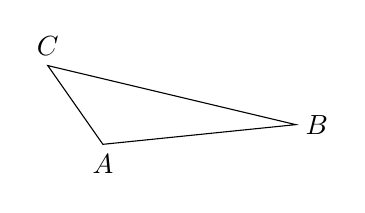
\begin{tikzpicture}[ xscale=0.7, yscale=0.5]
      \draw (0,0)--(3.5,0.5)--(-1,2)--cycle;
      \draw (0,0) node[below] {$A$};
      \draw (3.5,0.5) node[right] {$B$};
      \draw (-1,2) node[above] {$C$};
      \draw (0,-0.8) node {};
   \end{tikzpicture}
   &
   \propriete{} Dans un triangle, la somme des mesures des angles est égale à 180\degre.
   &
   Ici, $ABC$ est un triangle. \newline
   Donc $\widehat A+\widehat B + \widehat C= 180$\degre. \\ [-5mm]
   \hline %%%%%%%%%%%%%%%%%%%%%%P41
   \begin{tikzpicture}[ yscale=0.7]
      \draw (0,0)--(2,0)--(1,1.5)--cycle;
      \draw (0,0) node[left]{$A$};
      \draw (2,0) node[right]{$B$};
      \draw (1,1.5) node[above]{$C$};
      \draw (0.5,0.75) node[color=A1, rotate=146.31]{\large $\approx$};
      \draw (1.5,0.75) node[color=A1, rotate=56.31]{\large $\approx$};
      \draw (0,-0.4) node {};
   \end{tikzpicture}
   &
   \propriete{} Si un triangle est isocèle alors ses angles à la base ont la même mesure.
   &
   Ici, $ABC$ est isocèle en $C$. \newline
   Donc $\widehat A=\widehat B$. \\ [-5mm]
   \hline %%%%%%%%%%%%%%%%%%%%%%P42
   \begin{tikzpicture}[ scale=1.5]
      \draw (0,0)--(1,0)--(0.5,0.87)--cycle;
      \draw (0,0) node[left]{$A$};
      \draw (1,0) node[right]{$B$};
      \draw (0.5,0.87) node[above]{$C$};
      \draw (0.25,0.435) node[color=C1]{\large $\circ$};
      \draw (0.75,0.435) node[color=C1]{\large $\circ$};
      \draw (0.5,0) node[color=C1]{\large $\circ$};
      \draw (0,-0.2) node {};
   \end{tikzpicture}
   &
   \propriete{} Si un triangle est équilatéral alors ses angles mesurent 60\degre.
   &
   Ici, $ABC$ est équilatéral. \newline
   Donc $\widehat A = \widehat B = \widehat C = 60^\circ$. \\ [-5mm]
   \hline %%%%%%%%%%%%%%%%%%%%%%P43
   \begin{tikzpicture}[ xscale=0.5, yscale=0.4]
      \draw[fill=J1] (2,0.5)--(3,0) arc (-30:11.5:1.118)--(2,0.5)--(1,1) arc (150:191.5:1.118)--cycle;
      \draw (-1,-0.25)--(5,1.25); 
      \draw (-1,2)--(5,-1);
      \draw (2,0.5) node[above] {$A$};
      \draw (-1,-0.25) node[above] {$x$}; 
      \draw (-1,2) node[above] {$z$};
      \draw (5,1.25) node[above] {$y$}; 
      \draw (5,-1) node[above] {$t$};
      \draw (0,-1.8) node {};
   \end{tikzpicture}
   &
   \propriete{} Si deux angles sont opposés par le sommet alors ils ont la même mesure.
   &
   Ici, $\widehat{xAz}$ et $\widehat{yAt}$ sont opposés par le sommet. \newline
   Donc, $\widehat{xAz}=\widehat{yAt}$. \\ [-5mm]
   \hline %%%%%%%%%%%%%%%%%%%%%%P44
   \begin{tikzpicture}[ xscale=0.6,yscale=0.4]
      \draw [color=B1] (0,0)--(5,0.5);
      \draw [color=B1] (0,-1.5)--(5,-1);
      \draw (1,-2)--(5,1.5);
      \draw (0,0) node[above left] {$v$};
      \draw (0.8,-2) node[below] {$w$};
      \draw (5,1.5) node[above] {$z$};
      \draw (5,-1) node[below right] {$y$};
      \draw (1.8,-1.3) node[below right] {$E$};
      \draw (3.7,0.35) node[above left] {$G$};
      \draw [fill=J1] (1.8,-1.3)--(2.8,-1.2) arc (0:36:1)--cycle;
      \draw [fill=J1] (3.7,0.35)--(2.8,0.27) arc (180:213:1)--cycle; 
      \draw (0,-3.2) node{};
   \end{tikzpicture}
   &
   \propriete{} Si deux angles sont alternes-internes [resp. alternes-externes] compris entre des droites parallèles, alors ils ont même mesure. &
   Ici, $\widehat{vGw}$ et $\widehat{zEy}$ sont alternes-internes entre deux droites parallèles \newline
   Donc, $\widehat{vGw}=\widehat{zEy}$. \\ [-5mm]
   \hline %%%%%%%%%%%%%%%%%%%%%%P45
   \begin{tikzpicture}[ xscale=0.6,yscale=0.4] 
      \draw [color=B1] (0,0)--(5,0.5);
      \draw [color=B1] (0,-1.5)--(5,-1);
      \draw (1,-2)--(5,1.5);
      \draw (5,0.5) node[below right] {$t$};       
      \draw (5,1.5) node[above] {$z$};
      \draw (5,-1) node[below right] {$y$};
      \draw (1.8,-1.3) node[below right] {$E$};
      \draw (3.7,0.35) node[above left] {$G$};
      \draw[fill=J1] (1.8,-1.3)--(2.8,-1.2) arc (0:36:1)--cycle;
      \draw[fill=J1] (3.75,0.38)--(4.8,0.5) arc (0:38:1)--cycle; 
      \draw (0,-3.4) node{};
   \end{tikzpicture}
   &
   \propriete{} Si deux angles sont correspondants et que les droites sont parallèles alors ils ont la même mesure.
   &
   Ici, $\widehat{zGt}$ et $\widehat{zEy}$ sont correspondants et les droites sont parallèles. \newline
   Donc, $\widehat{zGt}=\widehat{zEy}$. \\ [-5mm]
   \hline %%%%%%%%%%%%%%%%%%%%%%P46
   \begin{tikzpicture}[ scale=0.2]
      \clip(-6,-10) rectangle (14,3);
      \draw [domain=-2.0:8] plot(\x,{(-52-2*\x)/12});
      \draw [domain=-2.0:8] plot(\x,{(-16--8*\x)/8});
      \draw [domain=-2:8, color=B2, very thick] plot(\x,{(-3.2--0.31*\x)/0.95});
      \draw (-2,-4) node[left] {$O$};
      \draw (9,-1.6) node[above] {$B$};
      \draw (4.9,3) node[below] {$x$};
      \draw (8,-5.8) node[above left] {$y$};
      \draw (3,-7.5) node {\footnotesize $[OB)$ est la bissectrice de $\widehat{xOy}$};
   \end{tikzpicture}
   &
   \propriete{} Si une droite est la bissectrice d'un angle alors elle partage l'angle en deux angles adjacents de même mesure.
   &
   Ici, $[OB)$ est la bissectrice de l'angle $\widehat{xOy}$. \newline
   Donc $\widehat{xOB}=\widehat{BOy}=\frac12\widehat{xOy}$. \\ [-5mm]
   \hline %%%%%%%%%%%%%%%%%%%%%%P47
   \begin{tikzpicture}[ scale=0.8]
      \draw (5.5,5.7) circle (1.5);
      \draw (4,5.7)--(4.6,6.9)--(6.65,4.75);
      \draw (4,5.7)--(5.5,5.7)--(6.65,4.75);
      \draw (4,5.7)--(6.5,6.8)--(6.65,4.75);
      \draw [fill=B2] (5.5,5.7)--(5.2,5.7)arc (180:320:0.3)--cycle;
      \draw [fill=J1] (4.6,6.9)--(4.35,6.4)arc (240:335:0.4)--cycle;
      \draw [fill=J1] (6.5,6.8)--(6.1,6.62)arc (210:281:0.4)--cycle;
      \draw [color=B2, very thick] (4,5.7)arc (180:320:1.5);
      \draw (4,5.7)node[left]{$A$};
      \draw (4.6,6.9)node[above left]{$B$};
      \draw (6.65,4.75)node[right]{$C$};
      \draw (6.5,6.8)node[right]{$D$};
      \draw (5.5,5.7)node[above left]{$O$};
      \draw (5,3.8) node {};
   \end{tikzpicture}
   &
   \propriete{} Si deux angles sont inscrits dans un même cercle et s'ils interceptent le même arc de cercle alors ils ont la même mesure et l'angle au centre qui intercepte le même arc de cercle mesure le double de l'angle inscrit.
   &
   Ici, les angles inscrits $\widehat{ABC}$ et $\widehat{ADC}$ ainsi que l'angle au centre $\widehat{AOC}$ interceptent le même arc $\wideparen{AC}$. \newline
   Donc, $\widehat{ABC} =\widehat{ADC} =\frac12\widehat{AOC}$. \\
   \hline
\end{tableau}


\subsection{Démontrer avec les droites remarquables du triangle}%J%

 
\begin{tableau}[pr]{\linewidth}
   \hline %%%%%%%%%%%%P48
   \begin{tikzpicture}[scale=0.9]
      \draw (0,0)--(2,0)--(0.5,1.5)--cycle;
      \draw (0,0) node[left]{$A$};
      \draw (2,0) node[right]{$B$};
      \draw (0.5,1.5) node[above]{$C$};
      \draw (0.5,0) node[below]{$D$};
      \draw [color=B2] (0.5,1.5)--(0.5,0);
      \draw [fill=G1] (0.5,0) rectangle (0.75,0.25);
      \draw (0,-0.5) node {};
   \end{tikzpicture}
   &
   \propriete{} Si, dans un triangle, une droite passe par un sommet et est perpendiculaire au côté opposé alors c'est une hauteur du triangle.
   &
   Ici, $(CD)\perp (AB)$. \newline
   Donc $(CD)$ est la hauteur issue de $C$ du triangle $ABC$ \\ [-6mm]
   \hline %%%%%%%%%%%%%%%%%%%%%%P49
   \begin{tikzpicture}[scale=0.9]
      \draw (0,0)--(2,0)--(0.5,1.5)--cycle;
      \draw (0,0) node[left]{$A$};
      \draw (2,0) node[right]{$B$};
      \draw (0.5,1.5) node[above]{$C$};
      \draw (1,0) node[below]{$D$};
      \draw [color=B2] (0.5,1.5)--(1,0);
      \draw (0.5,0) node[color=A1, rotate=90]{$\approx$};
      \draw (1.5,0) node[color=A1, rotate=90]{$\approx$};
      \draw (0,-0.5) node {};
   \end{tikzpicture}
   &
   \propriete{} Si, dans un triangle, une droite passe par un sommet et par le milieu du côté opposé alors c'est une médiane du triangle.
   &
   Ici, $D$ est le milieu de $[AB]$. \newline
   Donc, $[CD]$ est la médiane issue de $C$ du triangle $ABC$. \\ [-6mm]
   \hline %%%%%%%%%%%%%%%%%%%%%%P50 
   \begin{tikzpicture}[ yscale=0.2, xscale=0.25]
      \coordinate (A) at (2,7);
      \coordinate (B) at (0,0);
      \coordinate (C) at (10,0);
      \coordinate (A') at (5,0);
      \coordinate (B') at (6,3.5);
      \coordinate (C') at (1,3.5);
      \coordinate (G) at (4,2.3);  
      \draw (A)--(B)--(C)--cycle; 
      \draw[color=B2,dashed] (A)--(A'); 
      \draw[color=B2,dashed] (B)--(B'); 
      \draw[color=B2,dashed] (C)--(C'); 
      \foreach \N/\pos in {A/above, B/below left, C/below right, A'/below, B'/above right, C'/left, G/above} {\draw (\N) node[\pos] {$\N$};}
      \foreach \x/\y/\symb in {0.5/1.75/$\approx$, 1.5/5.25/$\approx$, 4/5.25/$\circ$, 8/1.75/$\circ$, 2.5/0/$|$, 7.5/0/$|$} {\draw[color=G1] (\x,\y) node {\small {\boldmath \symb}};}
      \draw (1,-3) node {};
   \end{tikzpicture}
   &
   \propriete{} Dans un triangle, les trois médianes sont concourantes en un point qui est le centre de gravité du triangle et qui se situe aux deux tiers des médianes en partant du sommet.
   &
   Ici, $G$ est le centre de gravité du triangle $ABC$ et $[AA']$ en est une médiane. \newline
   Donc $AG=\frac23AA'$. \\ [-4mm]
   \hline %%%%%%%%%%%%%%%%%%%%%%P51 
   {\psset{unit=0.65,linewidth=0.025}
   \begin{pspicture}(-0.8,-1.2)(5,3)
      \psset{CodeFig=true, PointSymbol=none,RightAngleSize=0.2}
      \pstTriangle{A}(4,0){B}(1.5,2.5){C}
      \pstProjection[PointName=none,CodeFigColor=B2]{B}{A}{C}
      \pstProjection[PointName=none,CodeFigColor=B2]{A}{C}{B}
      \pstProjection[PointName=none,CodeFigColor=black]{C}{B}{A}
      \rput(1.8,0.9){$H$}
   \end{pspicture}}
   &
   \propriete{} Dans un triangle, les trois hauteurs sont concourantes en un point appelé orthocentre du triangle.
   &
   Ici, $H$ est le point de concours de la hauteur issue de $C$ et de celle issue de $B$. \newline
   Donc, $[AH]$ est la hauteur issue de $A$. \\ [-6mm]
   \hline %%%%%%%%%%%%%%%%%%%%%%P52
   {\psset{unit=0.5,linewidth=0.025}
   \begin{pspicture}(-1.4,-2.7)(5,3.6)
      \psset{CodeFig=true,PointSymbol=none,linecolor=B2}
      \pstTriangle{A}(5,0){B}(1.5,3){C}
      \pstCircleABC[RightAngleSize=0.2,CodeFigColor=black]{A}{B}{C}{O}
   \end{pspicture}}
   &
   \propriete{} Dans un triangle, les trois médiatrices sont concourantes en un point qui est le centre du cercle circonscrit au triangle.
   &
   Ici, le cercle est circonscrit au triangle $ABC$. \newline
   Donc, son centre $O$ est le point de concours des médiatrices du triangle $ABC$. \\ [-6mm]
   \hline %%%%%%%%%%%%%%%%%%%%%%P53
   {\psset{unit=0.55,linewidth=0.025}
   \begin{pspicture}(-0.5,-1.5)(5,3.5)
      \psset{PointSymbol=none}
      \pstTriangle{A}(5,0){B}(1.5,3){C}
      \pstBissectBAC[linecolor=B2, PointName=none]{B}{A}{C}{A'}
      \pstBissectBAC[linecolor=B2, PointName=none]{A}{C}{B}{C'}
      \pstBissectBAC[linecolor=B2, PointName=none]{C}{B}{A}{B'}
      \pstMarkAngle[linecolor=J1, Mark=MarkHash, MarkAngleRadius=0.8]{B}{A}{A'}{}
      \pstMarkAngle[linecolor=J1, Mark=MarkHash, MarkAngleRadius=0.7]{A'}{A}{C}{}
      \pstMarkAngle[linecolor=J1, MarkAngleRadius=0.8]{C}{B}{B'}{}
      \pstMarkAngle[linecolor=J1, MarkAngleRadius=0.9]{B'}{B}{A}{}
      \pstMarkAngle[linecolor=J1, Mark=MarkCros, MarkAngleRadius=0.7]{A}{C}{C'}{}
      \pstMarkAngle[linecolor=J1, Mark=MarkCros, MarkAngleRadius=0.6]{C'}{C}{B}{}
      \pstInterLL{C}{C'}{A}{A'}{I}
      \pstProjection[PointName=none]{A}{B}{I}[I']
      \pstCircleOA[linestyle=dashed]{I}{I'}
   \end{pspicture}}
   &
   \propriete{} Dans un triangle, les trois bissectrices sont concourantes en un point qui est le centre du cercle inscrit au triangle.
   &
   Ici, le cercle est inscrit dans le triangle $ABC$. \newline
   Donc, son centre $I$ est le point de concours des bissectrices du triangle $ABC$. \\ [-4mm]
   \hline %%%%%%%%%%%%%%%%%%%%%%P58   
   \begin{tikzpicture}[ xscale=1.3, yscale=1.3]
      \draw (0,0)--(2,0)--(1,1.5)--cycle;
      \draw (0,0) node[left]{$A$};
      \draw (2,0) node[right]{$B$};
      \draw (1,1.5) node[above]{$C$};
      \draw (1,0) node[below]{$M$};
      \draw (0.5,0.75) node[color=C1]{ $\circ$};
      \draw (1.5,0.75) node[color=C1]{$\circ$};
      \draw (0.5,0) node[color=A1, rotate=90]{ $\approx$};
      \draw (1.5,0) node[color=A1, rotate=90]{$\approx$};
      \draw (1,1.5)--(1,0);
      \draw [fill=G1] (1,0)rectangle(1.2,0.2);
      \draw (1,-0.6) node {};
   \end{tikzpicture}
   &
   \propriete{} Si un triangle est isocèle, alors la médiane, la hauteur, la bissectrice issues du sommet principal et la médiatrice de la base sont confondues.
   &
   Ici, $ABC$ est isocèle en $C$, $M$ est le milieu de $[AB]$ et $(CM)\perp(AB)$. \newline
   Donc, $(CM)$ est la médiane, la hauteur, la bissectrice issue de $C$, la médiatrice de $[AB]$. \\
   \hline
\end{tableau}



%%%%%%%%%%%%%%%%%%%%%%%%%%%%%%%
%%%%%%%%%%%%%%%%%%%%%%%%%%%%%%%
\exercicesbase

\begin{center}
   {\cursive Maîtriser les bases avec} \href{http://mathenpoche.sesamath.net}{
\includegraphics[width=3cm]{Nombres_et_calculs/Images/mathenpoche}} \\
   \bigskip
   {\hautab{0.85}
   \cursive
   \begin{Ltableau}{0.775\linewidth}{4}{C{1}|C{1}|p{7cm}|p{2.3cm}}
      \hline
      Classe & \texttt{N\degre} & Thème & Dans le cours \\
      \hline
      \textcolor{orange}{\bf 6\up{e}} & \texttt{E1} & Bases de la géométrie plane & 1., 3. et 6. \\
      & \texttt{E2} & Parallèles et perpendiculaires & 1. et 6. \\
      & \texttt{E3} & Triangles & 4. \\
      & \texttt{E4} & Quadrilatères & 4. et 6. \\
      & \texttt{E6} & Médiatrice, bissectrice & 1. et 6. \\
      & \texttt{G2} & Angles & 2. et 6. \\
      \hline
      \textcolor{cyan}{\bf 5\up{e}} & \texttt{D1} & Angles et triangles & 1., 2. et 6. \\
      & \texttt{D2} & Transformation et parallélogramme & 4. et 6. \\
      \hline
      \textcolor{violet}{\bf 4\up{e}} & \texttt{D1} & Angles et triangles & 4. et 6. \\
      \hline
   \end{Ltableau}}
\end{center}

\bigskip


\begin{exercice}[Figures dynamisantes, ou pas !] %%% 1
   On considère les quadrilatère suivants :
   \begin{itemize}
      \item Un carré de 3 cm de côté.
      \item Un losange dont les diagonales mesurent 4 cm et 6 cm.
      \item Un parallélogramme dont un côté mesure 3 cm et l’autre 2 cm. \\ [-10mm]
   \end{itemize}
   \begin{enumerate}
      \item Tracer ces quadrilatères à l'aide d'un logiciel de géométrie dynamique.
      \item Tracer ces quadrilatères à la règle graduée et au compas. Y-a-t-il plusieurs configurations possibles ?
   \end{enumerate}
\end{exercice}

\begin{corrige}
   \ \\ [-5mm]
   \begin{enumerate}
      \item On peut pour cela utiliser un logiciel comme CarMetal ou GeoGebra, on construit pas à pas chacun des objets qui constituent les figures demandées en respectant les contrainte de mesure et d'orientation. \\
         L'aspect \og dynamique \fg{} permet de vérifier sa construction : en effet, si l'un des objets est mal construit et que l'on déplace l'un des points de la figure, celle-ci va se transformer.
      \item Pour les figures 1 et 2, il y a une seule configuration possible, à isométries près. \\
         Pour la figures 3, il y a une infinité de configurations qui dépendant de l'endroit où l'on place le troisième point. \\
         \begin{pspicture*}(-0.5,-0.5)(3.5,4)
            \pspolygon[fillstyle=solid,fillcolor=lightgray!50](0,0)(3,0)(3,3)(0,3)
            \psset{linecolor=gray}
            \pscircle(3,0){3}
            \psline(0,0)(0,4)
            \psline(3,0)(3,4)
            \psline(-1,3)(3,3)
            \rput(-0.3,-0.3){A}
            \rput(3.3,-0.3){B}
            \rput(3.3,3.3){C}
            \rput(-0.3,3.3){D}
         \end{pspicture*}
         \begin{pspicture*}(-3.7,-2.5)(3.5,2.5)
            \pspolygon[fillstyle=solid,fillcolor=lightgray!50](-3,0)(0,-2)(3,0)(0,2)
            \psset{linecolor=gray}
            \psline(-3,0)(3,0)
            \psline(0,-3)(0,3)
            \pscircle(0,0){2}
            \rput(-3.3,0){A}
            \rput(3.3,0){C}
            \rput(0.3,-2.3){B}
            \rput(0.3,2.3){D}
         \end{pspicture*}
         \begin{pspicture*}(-0.4,-0.5)(4.4,2.5)
            \pspolygon[fillstyle=solid,fillcolor=lightgray!50](0,0)(3,0)(3.9,1.8)(0.9,1.8)
            \psset{linecolor=gray}
            \pscircle(0,0){2}
            \pscircle(3,0){2}
            \pscircle(0.9,1.8){3}
            \rput(-0.3,0){A}
            \rput(3.3,0){B}
            \rput(1,2.2){D}
            \rput(4.2,2.1){C}
         \end{pspicture*}
   \end{enumerate}
\end{corrige}


\bigskip

\begin{exercice}[Construction d'un ove] %%% 6
   Voici un programme de construction d'un ove (motif ornemental en forme d'œuf qui orne une corniche ou une moulure).
   \begin{center}
      \fbox{\it
         \begin{minipage}{15cm}
         \medskip
            -- Soit $[AB]$ un segment et $I$ son milieu. \\
            -- Soit $C$ un point de la médiatrice de $[AB]$ tel que $IC = AB/2$. \\
            -- Tracer le triangle $ABC$. \\
            -- Tracer le petit arc de cercle de centre $B$ de rayon $AB$ délimité par les demi-droites $[BA)$ et $[BC)$. \\
            -- Appeler $E$ le point d'intersection de cet arc avec la droite $(BC)$. \\
            -- De même, tracer le petit arc de cercle de centre $A$ de rayon $AB$ par les demi-droites $[AB)$ et $[AC)$. \\
            -- Appeler $F$ le point d'intersection de cet arc avec la droite $(AC)$. \\
            -- Tracer le demi-cercle de diamètre $[AB]$ ne contenant pas $C$. \\
            -- Tracer l'arc de cercle $\wideparen{EF}$ de centre $C$ de rayon $EC$ entièrement situé à l'extérieur du triangle $ABC$. 
         \medskip
         \end{minipage}
      }
   \end{center}
   Tracer l'ove sur votre feuille en utilisant uniquement le compas et la règle non graduée. Laisser les traits de construction apparents et prendre pour longueur du segment $[AB]$ la longueur ci-dessous.
      \begin{center}
         {\psset{unit=0.8}
         \begin{pspicture}(0,0)(8,0.5)
            \psline{|-|}(0,0)(8,0)
            \rput(0,-0.4){$A$}
            \rput(8,-0.4){$B$}
         \end{pspicture}}
      \end{center}
\end{exercice}

\begin{corrige}
\ \\ [-5mm]
   {\psset{unit=0.8}
   \begin{pspicture}(-10,-5)(4,6)
      \pstGeonode[PosAngle={180,0,0,45}](-4,0){A}(4,0){B}(0,4){C}(0,0){I}
      \pstGeonode[PointName=none,PointSymbol=none](0,5){Z}(0,-5){Y}(0,4){X}
      \pstLineAB{A}{B}
      \pstLineAB[nodesepB=-3]{B}{C}
      \pstLineAB[nodesepB=-3]{A}{C}
      \pstInterLC[PointNameA=,PointSymbolA=none,PosAngleB=180]{B}{C}{B}{A}{E'}{E}
      \pstArcOAB[linewidth=0.7mm]{B}{E}{A}
      \pstInterLC[PointNameA=,PointSymbolA=none]{A}{C}{A}{B}{F'}{F}        
      \pstArcOAB[linewidth=0.7mm]{A}{B}{F}
       \pstArcOAB[linewidth=0.7mm]{I}{A}{B}
       \pstArcOAB[linewidth=0.7mm]{C}{F}{E}
       {\psset{arcsepA=-1.5,arcsepB=-2,linestyle=dashed}
          \pstArcOAB{A}{Z}{Z}
          \pstArcOAB{B}{Z}{Z}
          \pstArcOAB{A}{Y}{Y}
          \pstArcOAB{B}{Y}{Y}
          \pstLineAB{Y}{Z}
       }
   \end{pspicture}}
\end{corrige}


\bigskip


\begin{exercice}[Reproduire une figure - vers l'écriture d'un programme]
   On propose ci-dessous un programme de construction en six étapes principales. Les éléments en rouge sont les \og nouveautés \fg{} de chaque étape.
   \begin{center}
   {\footnotesize
      \begin{tabular}{C{7}C{8}}
         %\hline
            \begin{pspicture}(-3,-2.5)(2,2) %1
               \rput(-3,1.5){\large 1.}
               \color{red}{\psset{linecolor=red,linewidth=0.5mm}
                  \pstGeonode[PosAngle={180,-25,55}](0,0){O}(1.5;-25){M}(0.75;-25){I}
                  \pstCircleOA{O}{M}
                  \pstLineAB{O}{M}
                  \pstCircleOA{I}{M}
                  \rput(1.9;40){$\mathcal{(C)}$}
               }
            \end{pspicture}
            &
            \begin{pspicture}(-3,-2.5)(2,2) %2
               \rput(-3,1.5){\large 2.}
               \rput(1.9;40){$\mathcal{(C)}$}
               \pstGeonode[PosAngle={180,-25,55}](0,0){O}(1.5;-25){M}(0.75;-25){I}
               \pstCircleOA{O}{M}
               \pstLineAB{O}{M}
               \pstCircleOA{I}{M}
               \color{red}{\psset{linecolor=red,linewidth=0.5mm}
                  \pstGeonode[PosAngle={65,-115}](1.5;65){E}(1.5;-115){F}
                  \pstLineAB{E}{F}
                  \pstLineAB{F}{I}
                  \pstInterLC[PosAngleA=-100,PointSymbolB=none,PointNameB=]{F}{I}{I}{O}{J}{K}
               }
            \end{pspicture}
            \\ [4mm]
            \begin{pspicture}(-3,-2.5)(2,2) %3
               \rput(-3,1.5){\large 3.}
               \rput(1.9;40){$\mathcal{(C)}$}
               \pstGeonode[PosAngle={180,-25,55}](0,0){O}(1.5;-25){M}(0.75;-25){I}
               \pstCircleOA{O}{M}
               \pstLineAB{O}{M}
               \pstCircleOA{I}{M}
               \pstGeonode[PosAngle={65,-115}](1.5;65){E}(1.5;-115){F}
               \pstLineAB{E}{F}
               \pstLineAB{F}{I}
               \pstInterLC[PosAngleA=-100,PointSymbolB=none,PointNameB=]{F}{I}{I}{O}{J}{K}
                \color{red}{\psset{linecolor=red,linewidth=0.5mm}
                   \pstCircleOA{F}{J}
                   \pstInterCC[PosAngleA=170,PosAngleB=-45]{F}{J}{O}{M}{C}{B}
               }
            \end{pspicture}
            &
            \begin{pspicture}(-3,-3.5)(2,2) %4
               \rput(-3,1.5){\large 4.}
               \rput(1.9;40){$\mathcal{(C)}$}
               \pstGeonode[PosAngle={180,-25,55}](0,0){O}(1.5;-25){M}(0.75;-25){I}
               \pstCircleOA{O}{M}
               \pstLineAB{O}{M}
               \pstCircleOA{I}{M}
               \pstGeonode[PosAngle={65,-115}](1.5;65){E}(1.5;-115){F}
               \pstLineAB{E}{F}
               \pstLineAB{F}{I}
               \pstInterLC[PosAngleA=-100,PointSymbolB=none,PointNameB=]{F}{I}{I}{O}{J}{K}
               \pstCircleOA{F}{J}
               \pstInterCC[PosAngleA=170,PosAngleB=-45]{F}{J}{O}{M}{C}{B}
               \color{red}{\psset{linecolor=red,linewidth=0.5mm}
                  \pstCircleOA{C}{B}
                  \pstInterCC[PosAngleA=130]{C}{B}{O}{M}{D}{B}
               }
            \end{pspicture}
            \\ [9mm]
            \begin{pspicture}(-3,-3.5)(2,2) %5
               \rput(-3,1.5){\large 5.}
               \rput(1.9;40){$\mathcal{(C)}$}
               \pstGeonode[PosAngle={180,-25,55}](0,0){O}(1.5;-25){M}(0.75;-25){I}
               \pstCircleOA{O}{M}
               \pstLineAB{O}{M}
               \pstCircleOA{I}{M}
               \pstGeonode[PosAngle={65,-115}](1.5;65){E}(1.5;-115){F}
               \pstLineAB{E}{F}
               \pstLineAB{F}{I}
               \pstInterLC[PosAngleA=-100,PointSymbolB=none,PointNameB=]{F}{I}{I}{O}{J}{K}
               \pstCircleOA{F}{J}
               \pstInterCC[PosAngleA=170,PosAngleB=-45]{F}{J}{O}{M}{C}{B}
               \pstCircleOA{C}{B}
               \pstInterCC[PosAngleA=130]{C}{B}{O}{M}{D}{B}
               \color{red}{\psset{linecolor=red,linewidth=0.5mm}
                  \pstCircleOA{B}{C}
                  \pstInterCC[PosAngleB=40]{B}{C}{O}{M}{C}{A} 
               }
            \end{pspicture}
            &
            \begin{pspicture}(-3,-3.5)(2,2) %6
               \rput(-3,1.5){\large 6.}
               \rput(1.9;40){$\mathcal{(C)}$}
               \pstGeonode[PosAngle={180,-25,55}](0,0){O}(1.5;-25){M}(0.75;-25){I}
               \pstCircleOA{O}{M}
               \pstLineAB{O}{M}
               \pstCircleOA{I}{M}
               \pstGeonode[PosAngle={65,-115}](1.5;65){E}(1.5;-115){F}
               \pstLineAB{E}{F}
               \pstLineAB{F}{I}
               \pstInterLC[PosAngleA=-100,PointSymbolB=none,PointNameB=]{F}{I}{I}{O}{J}{K}
               \pstCircleOA{F}{J}
               \pstInterCC[PosAngleA=170,PosAngleB=-45]{F}{J}{O}{M}{C}{B}
               \pstCircleOA{C}{B}
               \pstInterCC[PosAngleA=130]{C}{B}{O}{M}{D}{B}
               \pstCircleOA{B}{C}
               \pstInterCC[PosAngleB=40]{B}{C}{O}{M}{C}{A} 
               \color{red}{\psset{linecolor=red,linewidth=0.5mm}
                  \pstLineAB{A}{B}
                  \pstLineAB{B}{C}
                  \pstLineAB{C}{D}
                  \pstLineAB{D}{E}
                  \pstLineAB{E}{A}
               }
            \end{pspicture} \\ [2mm]
            %\hline
      \end{tabular}}
   \end{center}
   \begin{enumerate}
      \item Reproduire cette figure sur votre feuille.
      \item Quelle figure construit-on grâce à ce programme (aucune justification n'est demandée).
      \item Écrire un programme de construction correspondant à ces six étapes.
   \end{enumerate}
\end{exercice}

\begin{corrige}
\ \\ [-5mm]
   \begin{enumerate}
      \setcounter{enumi}{1}
      \item La figure construite est un {\blue pentagone régulier}.
      \item Étape 1 : tracer un cercle $(\mathcal{C})$ de centre $O$ et un rayon $[OM]$. \\
         Tracer le cercle de diamètre $[OM]$ de centre $I$. \\
         Étape 2 : tracer le diamètre $[EF]$ de $(\mathcal{C})$ perpendiculaire à $(OM)$. \\
         Tracer le segment $[IF]$, il coupe le cercle de centre $I$ et de rayon $IO$ et $J$. \\
         Étape 3 : tracer le cercle de centre $F$ passant par $J$, il coupe le cercle $(\mathcal{C})$ aux points $B$ et $C$, $B$ étant le point le plus proche de $M$. \\
         Étape 4 : tracer le cercle de centre $C$ passant par $B$, il recoupe le cercle $(\mathcal{C})$ en $D$. \\
         Étape 5 : tracer le cercle de centre $B$ passant par $C$, il recoupe le cercle $(\mathcal{C})$ en $A$. \\
         Étape 6 : tracer le pentagone $ABCDE$.
   \end{enumerate}
\end{corrige}


\pagebreak

\begin{exercice}[CRPE 2008 G1] %%% 8   
   Le syndicat d'initiative de la ville de Bellerive organise une chasse au trésor. Voici ci-dessous les indices recueillis par les concurrents. Sur le schéma page suivante figure le plan des lieux de la chasse au trésor.
   \begin{itemize}
      \item Indice 1 : Le trésor se trouve à plus de 500 mètres de la ligne à haute tension L.
      \item Indice 2 : Le trésor est à plus de 800 mètres de l'école E.
      \item Indice 3 : Le trésor se trouve à moins de 300 mètres de la bibliothèque B.
      \item Indice 4 : Le trésor est à égale distance du stade S et de la piscine P.
   \end{itemize}
   Pour les quatre questions suivantes, aucune construction n'est demandée, seule la description des régions correspondantes dans la réalité est demandée.
   \begin{enumerate}
      \item En considérant l'indice 1, caractériser la région du plan dans laquelle le trésor peut se trouver.
      \item En considérant l'indice 2, caractériser la région du plan dans laquelle le trésor peut se trouver.
      \item En considérant l'indice 3, caractériser la région du plan dans laquelle le trésor peut se trouver.
      \item En considérant l'indice 4, caractériser la région du plan dans laquelle le trésor peut se trouver.
      \item Pour cette question, une construction géométrique est attendue. Elle doit être réalisée sur la copie à la règle graduée, à l'équerre et au compas. \\
      Le plan représenté page suivante est à l'échelle $\dfrac{1}{10\,000}$. \\
      Reproduire ce plan sur votre copie sachant que :
      \begin{itemize}
         \item les points E et B sont situés à 5 cm de la droite L avec EB = 6 cm ;
         \item le triangle EBS est isocèle en B avec ES = 10 cm ;
         \item P est le milieu du segment [ES].
      \end{itemize}
      Mettre en évidence, avec une autre couleur par exemple, la partie du plan dans laquelle se trouve le trésor. Tous les tracés nécessaires à cette construction seront laissés apparents.
   \end{enumerate}
   \begin{center}
      \begin{pspicture}(-1,-3.75)(15,7.25)
      \psset{algebraic=true}
         \psplot{-1}{13}{(--27.3276--2.04*x)/7.78}
         \rput[bl](4.1,5){L}
         \psdots[dotstyle=x](10.1,1)(4.3,-0.5)(13.7,-3.8)(9,-2.15)
         \rput[bl](10.3,0.6){B}
         \rput[bl](4.5,-0.9){E}
         \rput[bl](13.9,-4.3){S}
         \rput[bl](9.1,-2){P}
      \end{pspicture}
   \end{center}
\end{exercice}

\begin{corrige}
\ \\ [-5mm]
   \begin{enumerate}
      \item La région correspondant à l'indice 1 est constituée de deux demi-plans dont les frontières sont des droites parallèles, de part et d'autre de L et situées à 500 mètres de L.
      \item La région correspondant à l'indice 2 est l'extérieur du cercle de centre E et de rayon 800 mètres.
      \item La région correspondant à l'indice 3 est l'intérieur du cercle de centre B et de rayon 300 mètres.
      \item La région correspondant à l'indice 4 est la médiatrice du segment [SP].
      \item L'échelle est 1/10\,000\up{e} : 1 cm sur la figure représente 10 000 cm dans la réalité, c'est-à-dire 100 m.
   \end{enumerate}
   Sur la figure suivante, le trésor se trouve sur le segment rouge. \\
   \begin{center}
      \begin{pspicture*}(0,-4)(16,8)
      \psset{algebraic=true}
         \psplot{-1}{15}{(--27.33--2.04*x)/7.78}
         \rput[bl](4.1,5){L}
         \psdots[dotstyle=+](10.1,1)(4.3,-0.5)(13.7,-3.8)(9,-2.15)
         \rput[bl](10.3,0.6){B}
         \rput[bl](4.5,-0.9){E}
         \rput[bl](13.9,-4.3){S}
         \rput[bl](9.1,-2){P}
         \psline[linewidth=2mm,linecolor=B2](12.3,-0.3)(13,1.7)
         \psset{linecolor=A1}
         \psplot{-1}{15}{(-12.89--2.04*x)/7.78}
         \psplot{-1}{15}{(--67.54--2.04*x)/7.78}
        \pscircle(4.3,-0.5){8}
         \pscircle(10.1,1){3}
         \psplot{-12.3}{24.2}{(-58.55--4.73*x)/1.62}      
      \end{pspicture*}
   \end{center}
\end{corrige}


\bigskip

\begin{exercice}[Les bandelettes] %%% 1
   {\it Exercice issu du site de \href{http://pernoux.pagesperso-orange.fr/revision/revgeo.pdf}{\bf Dominique Pernoux} - http://pernoux.pagesperso-orange.fr/revision/revgeo.pdf}. 
   
   On fabrique à l'aide de bandelettes de bristol des \og squelettes \fg{} de quadrilatères : chaque squelette est composé de deux bandelettes fixées \og en croix \fg{} à l'aide d'une attache parisienne qui les traverse aux endroits notés O, O' et I (situés au centre de la bandelette). Aux emplacements désignés par les lettres M, N, P, Q, R, S on a percé des trous permettant de passer la mine d'un crayon pour tracer les points correspondants, sommets du quadrilatère dont les diagonales sont matérialisées par le \og squelette \fg. \\
   On dispose de deux types de bandelettes de deux longueurs différentes, semblables à celles représentées ci-dessous.
   \begin{center}
      \begin{pspicture}(0,-1.5)(11,2)
         \psframe[linewidth=2pt](0,0)(11,1.4)
         \pstGeonode[PosAngle=-90,PointNameSep=8pt](1,0.7){M}(10,0.7){N}(5.5,0.6){O}(7.5,0.6){O'}
         \pscircle[linewidth=6pt](5.5,0.7){0.1}
         \pscircle[linewidth=6pt](7.5,0.7){0.1}
         \psline{|-|}(1,1.7)(10,1.7)
         \rput(5.5,2){9 cm}
         \psline{|-|}(5.5,-0.3)(7.5,-0.3)
         \rput(6.5,-0.6){2 cm}
      \end{pspicture}

      \begin{pspicture}(0,-1.5)(11,1.5)
         \psframe[linewidth=2pt](0,0)(11,1.4)
         \pstGeonode[PosAngle=-90,PointNameSep=8pt](1,0.7){P}(10,0.7){Q}(5.5,0.6){O}(7.5,0.6){O'}
         \pscircle[linewidth=6pt](5.5,0.7){0.1}
         \pscircle[linewidth=6pt](7.5,0.7){0.1}
      \end{pspicture}

      \begin{pspicture}(0,-0.5)(7,1.5)
         \psframe[linewidth=2pt](0,0)(7,1.4)
         \pstGeonode[PosAngle=-90,PointNameSep=8pt](1,0.7){R}(6,0.7){S}(3.5,0.6){I}
         \pscircle[linewidth=6pt](3.5,0.7){0.1}
         \psline{|-|}(1,1.7)(6,1.7)
         \rput(3.5,2){5 cm}
      \end{pspicture}
   \end{center}
   \begin{enumerate}
      \item On considère un \og squelette \fg{} obtenu en prenant deux grandes bandes et en les faisant se croiser toutes les deux au point O. On s'intéresse aux quadrilatères MQNP tracés à partir de ce \og squelette \fg{}. \\
      Quelle famille de quadrilatères peut-on obtenir par ce procédé ? Identifier les cas particuliers éventuels. Justifier.
      \item On considère un squelette obtenu en faisant se croiser une petite bande au niveau du point I et une grande bande au niveau du point O. On s'intéresse aux quadrilatères MSNR tracés à partir de ce \og squelette \fg{}. \\
         Quelle famille de quadrilatères peut-on obtenir par ce procédé ? Identifier les cas particuliers éventuels. Justifier.
      \item On considère un squelette obtenu en faisant se croiser une petite bande au niveau du point I et une grande bande au niveau du point O'. \\
         Construire à la règle graduée un quadrilatère MSNR de cette famille. Démontrer qu'il possède un angle droit.
      \item On considère un squelette obtenu en prenant deux grandes bandes et en les croisant l'une au niveau du point O, l'autre au niveau du point O'. \\
         Construire à la règle graduée et au compas un quadrilatère MQNP de cette famille qui possède un angle droit.
   \end{enumerate}
\end{exercice}

\begin{corrige}
\ \\ [-5mm]
   \begin{enumerate}
      \item Les diagonales du quadrilatère QMNP sont [MN] et [PQ]. Ces diagonales sont de même longueur et se coupent en O, le milieu de [MN] et de [PQ].  Ce procédé permet de construire {\blue une famille de rectangles}. \\
         Cas particulier : lorsque les diagonales sont perpendiculaires, on obtient un {\blue carré}.
      \item Les diagonales du quadrilatère MSNR sont [MN] et [RS]. Ces diagonales se coupent en O = I, milieu de [MN] et de [RS]. Ce procédé permet de construire {\blue une famille de parallélogrammes}. \\
         Cas particulier : lorsque les diagonales sont perpendiculaires, on obtient un {\blue losange}.
      \item Programme de construction : \\
         \begin{itemize}
            \item Construire le segment [MN] de longueur \ucm{9} ainsi que le point O' sur ce segment situé à \ucm{2,5} de N ;
            \item tracer le segment [RS] de longueur \ucm{5} et de milieu O' ;
            \item tracer le quadrilatère MSNR.
         \end{itemize}
         {\psset{unit=0.9}
         \begin{pspicture}(-5,0.5)(9,5.5)
            \pspolygon[linecolor=B2](1,1)(5.5,4.6)(9.6,3.5)(8.9,1)
            \pspolygon[linecolor=A1](9.2,3.6)(9.1,3.2)(9.5,3.1)(9.6,3.5)
            \psline(1,1)(9.6,3.5)
            \pscircle(7.2,2.8){2.5}
            \psline(5.5,4.6)(8.9,1)
            \rput[bl](0.5,0.9){M}
            \rput[bl](9.82,3.64){N}
            \rput[bl](7.1,3.2){O'=I}
            \rput[bl](5.26,4.9){R}
            \rput[bl](9.08,0.72){S}
         \end{pspicture}}
         \bigskip \\
         On a I = O' donc, dans le quadrilatère MSNR, O'R = O'N = O'S et O' est le milieu de [RS] d'où : N est sur le cercle de diamètre [RS] ce qui implique que le triangle SNR est rectangle en N. \\
         {\blue Le quadrilatère MSNR possède donc un angle droit en N}.
      \item Programme de construction : \\
         \begin{itemize}
            \item Construire le segment [MN] de longueur 9 cm ainsi que le point O' sur ce segment situé à \ucm{2,5} de N ;
            \item tracer le cercle de diamètre [MN] et le cercle de centre O' et de  rayon \ucm{4,5} : placer P sur l'un des points d'intersection de ces cercles ;
            \item construire Q sur la droite (PO') tel que PQ = \ucm{9} ;
            \item tracer le quadrilatère MQNP. \\
         \end{itemize}
      {\psset{unit=0.6}
      \begin{pspicture}(-10,-2.2)(12,8)
         \pspolygon[linecolor=A1](4.6,6.3)(5.1,6)(5.4,6.5)(4.9,6.8)
         \psline(1,1)(9.6,3.7)
         \pscircle(5.3,2.35){4.5}
         \pscircle(7.2,2.95){4.5}
         \pspolygon[linecolor=B2](1,1)(4.9,6.8)(9.6,3.7)(9.5,-0.9)      
         \psline(4.9,6.8)(9.5,-0.9)
         \rput[bl](0.2,0.85){M}
         \rput[bl](9.8,3.9){N}
         \rput[bl](7.2,3.2){O'}
          \rput[bl](5,7.2){P}
        \rput[bl](9.3,-1.7){Q}
      \end{pspicture}}
      \bigskip \\
      Le point P est situé sur le cercle de diamètre [MN], donc le triangle MNP est rectangle en P. \\
      {\blue Le quadrilatère MPNQ possède donc un angle droit en P}.
   \end{enumerate}
\end{corrige}


\pagebreak


\begin{exercice}[Portrait de quadrilatères] %%%% 2
   Voici un jeu tiré de {\it Géométrie à l'École} de François Boule, Savoir dire et savoir-faire, IREM de Bourgogne. \\
   Il est constitué de dix étiquettes. \medskip
   \begin{center}
      {\hautab{1.2}
      \begin{tabular}{C{7}C{7}}
         \fbox{Deux angles droits seulement} & \fbox{Quatre angles droits} \\
         & \\
         \fbox{Côtés égaux deux à deux} & \fbox{Deux côtés égaux seulement} \\
         & \\
         \fbox{Quatre côtés égaux} & \fbox{Côtés opposés parallèles} \\
         & \\
         \fbox{Deux côtés parallèles seulement} & \fbox{Diagonales égales} \\
         & \\
         \fbox{Diagonales perpendiculaires} & \fbox{Diagonales se croisant en leur milieu} \\
      \end{tabular}} \medskip
   \end{center}
   On choisit au hasard deux étiquettes parmi les dix et on doit essayer de dessiner un quadrilatère qui a ces deux propriétés.
   \begin{enumerate}
      \item Un enfant a sélectionné les deux étiquettes suivantes : \fbox{ Deux angles droits seulement} et \fbox{ Diagonales perpendiculaires} \\ [-4mm]
      \begin{enumerate}
         \item En se limitant à la première propriété \og Deux angles droits seulement \fg, tracer à main levée les deux configurations possibles.
         \item En prenant en compte les deux propriétés, construire à l'aide des outils usuels de géométrie (règle, équerre, compas) une figure correspondant à chacune des deux configurations possibles.
        \item Rédiger les deux programmes de construction. \smallskip
      \end{enumerate}
      \item On choisit l’étiquette : \fbox{ Deux côtés parallèles seulement} \\ [1mm]
         Trouver toutes les étiquettes incompatibles avec elle. Justifier les réponses.
   \end{enumerate}
\end{exercice}

\begin{corrige}
\ \\ [-5mm]
   \begin{enumerate}
      \item 
         \begin{enumerate}
            \item On a les deux configurations suivantes selon si les angles droits sont consécutifs ou non : \\
               \begin{pspicture}(-3,-0.2)(8,3.5)
                  \pspolygon(0,0)(3,0)(2,2)(0,2)
                  \psframe(0,0)(0.3,0.3)  
                  \psframe(0,2)(0.3,1.7)
                  \rput(1.25,1){1}
                  \pspolygon(4,0)(8,0)(5,3)(4,2)
                  \psframe(4,0)(4.3,0.3)  
                  \pspolygon(5,3)(5.2,2.8)(5,2.6)(4.8,2.8)
                  \rput(5.5,1){2} 
               \end{pspicture}
            \item En ajoutant la deuxième contrainte, on obtient : \\
               \begin{minipage}{8cm}
                  \begin{pspicture}(-1,-0.7)(4,3.2)
                     \pspolygon[linewidth=0.5mm](0,0)(3,0)(1.33,2)(0,2)
                     \rput(-0.3,-0.3){A}
                     \rput(3.3,-0.3){B}
                     \rput(-0.3,2.3){D}
                     \rput(1.25,2.3){C}
                     \psframe(0,0)(0.3,0.3)  
                     \psframe(0,2)(0.3,1.7)
                     \psline(0,2)(3,0)
                     \psline(0,0)(2,3)
                     \psline(0,2)(3,2)
                     \rput{-123}(0.92,1.38){\psframe(0,0)(0.3,0.3)}
                  \end{pspicture}
               \end{minipage}
               \begin{minipage}{8cm}
                  \begin{pspicture}(-1,-0.8)(4,3)
                     \pspolygon[linewidth=0.5mm](0,0)(3,0)(1.85,2.77)(0,2)
                     \rput(-0.3,-0.3){A}
                     \rput(3.3,-0.3){B}
                     \rput(-0.3,2.3){D}
                     \rput(2.2,2.8){C}
                     \psframe(0,0)(0.3,0.3)  
                     \psline(0,2)(3,0)
                     \psline(0,0)(2,3)
                     \rput(0.46,0.69){\bf+}
                     \rput(1.38,2.08){\bf+}
                     \rput{-123}(0.92,1.38){\psframe(0,0)(0.3,0.3)}
                  \end{pspicture}
               \end{minipage}
           \item Programmes de construction : \\ [1mm]
              \begin{minipage}{8cm}
                  \begin{itemize}
                     \item Tracer un segment [AB].
                     \item Tracer un segment [AD] perpendiculaire à (AB).
                     \item Tracer le segment [BD].
                     \item Placer le point C à l'intersection de la droite perpendiculaire à (AD) passant par D et de la perpendiculaire à (BD) passant par A.
                     \item Tracer le quadrilatère ABCD. \\
                  \end{itemize}
               \end{minipage}
               \begin{minipage}{8cm}
                  \begin{itemize}
                     \item Tracer un segment [AB].
                     \item Tracer un segment [AD] perpendiculaire à (AB).
                     \item Tracer le segment [BD].
                     \item Placer le point C symétrique du point A par rapport à (BD).
                    \item Tracer le quadrilatère ABCD. \\ [6mm]
                  \end{itemize}
               \end{minipage}
         \end{enumerate}
         \setcounter{enumi}{1}
         \item Compatibilité avec l'étiquette \fbox{Deux côtés parallèles seulement} :
         \begin{itemize}
            \item \fbox{Deux angles droits seulement} : oui, tout trapèze rectangle qui n'est pas un rectangle convient. \medskip
            \item \fbox{Côtés égaux deux à deux} : oui, si ABCD est un rectangle, ABDC est un quadrilatère croisé qui convient. \medskip
            \item \fbox{Quatre côtés égaux} : non, un quadrilatère à quatre côtés égaux est un losange, dont les côtés opposés sont parallèles deux à deux. \medskip
            \item \fbox{Diagonales perpendiculaires} : oui, le trapèze rectangle de la configuration 1, question (b) convient. \medskip        
            \item \fbox{Quatre angles droits} : non, un quadrilatère à quatre angles droits est un rectangle, dont les côtés opposés sont parallèles  deux à deux. \medskip
            \item \fbox{Deux côtés égaux seulement} : oui, un trapèze dont deux côtés consécutifs sont égaux et dont les autres côtés ont des mesures différentes convient. \medskip
            \item \fbox{Côtés opposés parallèles} : non, implicitement, cela veut dire que les côtés opposés sont parallèles deux à deux. \medskip
            \item \fbox{Diagonales égales} : oui, un trapèze isocèle non rectangle convient. \medskip
            \item \fbox{Diagonales se rencontrant en leur milieu} : non, un quadrilatère dont les diagonales se coupent en leur milieu est un parallélogramme, dont les côtés opposés sont parallèles deux à deux.
         \end{itemize}
   \end{enumerate}
\end{corrige}


\bigskip

\begin{exercice}[CRPE 2006 G1] %%% 6
   ABC est un triangle tel que $\widehat{\text{A}} =$ 60\degre et $\widehat{\text{B}} =$ 45\degre. H est le pied de la hauteur issue de C. \\
   Le cercle de diamètre [AB] de centre I coupe (AC) en L et (BC) en K ; (AK) et (BL) se coupent en O.
   \begin{enumerate}
      \item 
         \begin{enumerate}
            \item Reproduire ce segment sur votre copie. \\
               \begin{pspicture}(-3,-1)(8,2)
                  \psline{|-|}(0,0)(8,1)
                  \rput(0,0.5){A}
                  \rput(8,0.5){B}
               \end{pspicture}
            \item À partir de ce segment et en utilisant uniquement la règle et le compas, terminer la construction d'un triangle ABC tel que $\widehat{\text{A}} =$ 60\degre et $\widehat{\text{B}} =$ 45\degre. Laisser apparents tous les traits de construction. 
         \end{enumerate}
      \item Démontrer que la droite (KI) est la médiatrice du segment [AB].
      \item Démontrer que les points C, O, H sont alignés.
      \item Quelle est la nature du quadrilatère IKCO ? Justifier votre réponse.  
   \end{enumerate}
\end{exercice}

\begin{corrige}
\ \\ [-5mm]
   \begin{enumerate}
      \item \textcolor{G1}{$\bullet$} Pour construire un angle de \udeg{60}, il suffit de construire un triangle équilatéral ;
         \begin{itemize}
            \item  pour construire un angle de \udeg{45}, on peut construire un angle droit grâce à une perpendiculaire, puis construire sa bissectrice. \\ [3mm]
            \end{itemize}
            {\psset{algebraic=true,unit=1.34}
            \begin{pspicture*}(-3,-1)(7,5.5)
               \pspolygon[linecolor=gray](0,0)(6,0)(3,5.2)
               \psline[linecolor=gray](6,-1)(6,6)
               \psplot[linecolor=gray]{-1}{7}{(-4.24--0.71*x)/-0.71}
               \psline[linecolor=B2](2.2,-1)(2.2,6)
               \pscircle(3,0){3}
               \psplot[linecolor=A1]{-1}{7}{--x}
               \psplot[linecolor=A1]{-1}{7}{(--16-2.6*x)/4.5}
               \psline[linecolor=G1](3,-0.5)(3,5.7)
               \pspolygon[linecolor=B2](0,0)(6,0)(2.2,3.8)
               \rput(-0.3,0){A}
               \rput[bl](6.1,0.2){B}
               \rput[bl](2.3,4){C}
               \rput[bl](0.6,0.2){\textcolor{B2}{60\degre}}
               \rput[bl](4.6,0.2){\textcolor{B2}{45\degre}}
              \rput[bl](2.28,-0.3){H}
               \rput[bl](3.08,-0.3){I}
               \rput[bl](1.5,2.8){L}
               \rput[bl](3.08,3.12){K}
               \rput[bl](2.28,2.32){O}
            \end{pspicture*}}
         \item
            \begin{itemize}
               \item I est le centre du cercle de diamètre [AB], il est donc situé au milieu de [AB], à égale distance de A et de B ;
               \item K est situé sur le cercle de diamètre [AB], le triangle ABK est inscrit dans un cercle ayant pour diamètre un de ses côtés, c'est donc un triangle rectangle en K. \\
                  Dans ce triangle, sachant que la somme des angles mesure 180\degre, que $\widehat{\text{ABK}}=45$\degre et $\widehat{\text{BKA}}=90$\degre, alors $\widehat{\text{KAB}}=180^\circ-90^\circ-45^\circ =45^\circ$. \\
                  Le triangle ABK est donc rectangle et isocèle en K puisqu'il possède deux angles de même mesure.
            \end{itemize}
            On a alors KA = KB, et IA = IB, donc, {\blue la droite (KI) est la médiatrice du segment [AB].}
         \item
            \begin{itemize}
                \item Le triangle ABK étant rectangle en K, la droite (AK) est perpendiculaire à la droite (BC). \\
                   (AK) est donc la hauteur issue de A du triangle ABC ;
                \item le triangle ABL étant rectangle en L (il est inscrit dans le cercle de diamètre [AB]), la droite (BL) est perpendiculaire à la droite (AC). (BL) est donc la hauteur issue de B du triangle ABC ;
                \item ces deux hauteurs se coupent en l'orthocentre noté O. La troisième hauteur du triangle ABC est la droite (CH), qui passe donc elle aussi par O.
            \end{itemize}     
            D'où : {\blue les points C, O, H sont alignés.}
         \item 
            \begin{itemize}
               \item (KI) est la médiatrice du segment [AB], donc, (KI) est perpendiculaire à (AB) ;
               \item (CH) est une hauteur du triangle ABC, donc, (CH) est perpendiculaire à (AB) ;
            \end{itemize}
            or, deux droites perpendiculaires à une même droite sont parallèles entre elles, donc, les droites (CH) et (KI) sont parallèles. D'après la question 2, O est un point de la droite (CH), d'où  (CO) et (KI) sont parallèles, d'où : \\
            {\blue le quadrilatère IKCO est un trapèze.}
   \end{enumerate}
\end{corrige}


\bigskip

\begin{exercice}[CRPRE 2008 G3] %%% 4
   ABC est un triangle dans lequel l'angle de sommet A est aigu. \\
   On considère le cercle de diamètre [BC]. Il coupe les droites (AB) et (AC) respectivement en D et E. \\
   Les droites (BE) et (CD) se coupent en H.
   \begin{enumerate}
      \item Faire une figure.
      \item Démontrer que les droites (AH) et (BC) sont perpendiculaires.
      \item Construire sur votre figure, avec la règle non graduée et le compas, le point M, quatrième sommet du parallélogramme BCMA et le point N, quatrième sommet du parallélogramme BCAN. \\
      On laissera les traits de construction apparents.
      \item Démontrer que le point A est le milieu de [MN].
   \end{enumerate}
\end{exercice}

\begin{corrige}
\ \\ [-5mm]
   \begin{enumerate}
      \item Exemple de figure de l'exercice :
         {\psset{algebraic=true,unit=0.9}
         \begin{pspicture*}(-7,-5.7)(8,6)
            \pspolygon(6,0)(2,5)(-4,5)(0,0)
            \pspolygon(6,0)(2,5)(0,0)(4,-5)
            \pscircle[linecolor=A1](4.,2.5){3.2015621187164243}
            \psplot[linecolor=B2]{-5}{8}{(--12.4-2.1*x)/5.17}
            \psline[linecolor=B2](2,-6)(2,6)
            \psplot[linecolor=B2]{-5}{8}{--0.8*x}
            \rput[bl](-0.6,-0.1){A}
            \rput[bl](6.4,0){B}
            \rput[bl](2.1,5.3){C}
            \rput[bl](2.1,0.1){D}
            \rput[bl](0.4,2.4){E}
            \rput[bl](2.1,1.9){H}
            \rput[bl](-4.6,5.1){M}
            \rput[bl](3.9,-5.6){N}
         \end{pspicture*}}
      \item
      \begin{itemize}
         \item D est un point du cercle de diamètre [BC] ; donc, le triangle BCD est rectangle en D et la droite (CD) est perpendiculaire à la droite (AB). D'où, (CD) est la hauteur issue de C du triangle ABC ;
         \item E est un point du cercle de diamètre [BC] ; donc, le triangle BCE est rectangle en E et la droite (BE) est perpendiculaire à la droite (AC). D'où, (BE) est la hauteur issue de B du triangle ABC ;
      \end{itemize}
      or, les hauteurs d'un triangle sont concourantes au point H appelé orthocentre. La troisième hauteur étant (AH), elle est perpendiculaire à la droite (BC). \\
      {\blue Les droites (AH) et (BC) sont perpendiculaires.}
   \item Voir figure.
   \item
      \begin{itemize}
         \item Le quadrilatère BCMA est un parallélogramme, donc, les droites (BC) et (AM) sont parallèles, et les segments [BC] et [AM] sont de même longueur ;
         \item le quadrilatère BCAN est un parallélogramme, donc, les droites (BC) et (NA) sont parallèles, et les segments [BC] et [NA] sont de même longueur ;
      \end{itemize}
      les droites (AM) et (NA) sont toutes les deux parallèles à (BC), elles sont donc parallèles entre elles et contiennent un point en commun ; par conséquent, elles sont confondues et les points M, A et N sont alignés dans cet ordre. \\
      De plus, les longueurs des segments [AM] et [NA] sont égales à la longueur du segment [BC], soit AM = AN, ce qui signifie que soit M et N sont confondus, soit A est au milieu de [MN]. Or, M et N ne peuvent pas être confondus par construction de BC{\bf MA} et BC{\bf AN}. \\
      Conclusion : {\blue le point A est le milieu du segment [MN].}
   \end{enumerate}
\end{corrige}


\bigskip

\begin{exercice}[CRPE 2014 G1 et 2018 G1] %%% 8
   Les affirmations suivantes sont-elles vraies ou fausses ?
   \begin{enumerate}
      \item La somme des angles d'un pentagone convexe est égale à \udeg{540}.
      \item Soit la figure ci-dessous faite à main levée. Les points $C, D$ et $E$ sont alignés.\\
         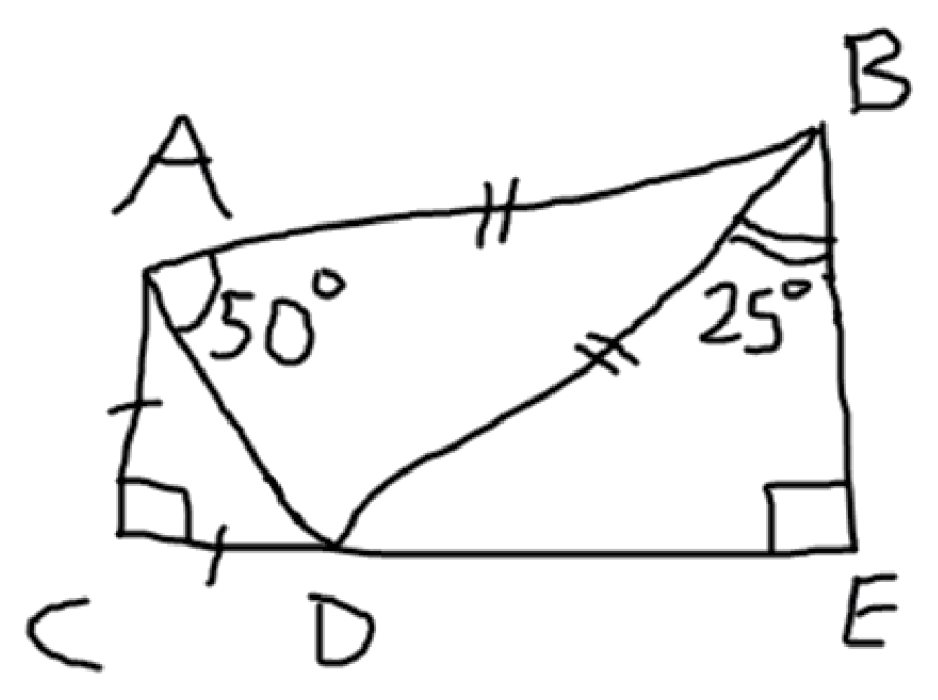
\includegraphics[width=4cm]{Geometrie/Images/G9_ex_angles}
   \end{enumerate}
\end{exercice}

\begin{corrige}
\ \\ [-5mm]
   \begin{enumerate}
      \item On a par exemple la figure suivante : \\
         \begin{pspicture}(-2,0)(5,4)
            \pstGeonode[CurveType=polygon,PosAngle={180,0,45,90,135}](0.5,0.5){A}(3,1){B}(3,3){C}(2,3){D}(0,2){E}
            \pstLineAB[linecolor=B2]{A}{C}
            \pstLineAB[linecolor=B2]{A}{D}
         \end{pspicture} \\
         Tout pentagone convexe $ABCDE$ peut être décomposé en trois triangles, par exemple  $BAC$, $CAD$ et $DAE$. \\
         Or, la sommes des angles d'un triangle vaut $180$\degre. \\
         La somme des angles du pentagone vaut donc $3\times\udeg{180} =\udeg{540}$. \\
         L'affirmation est {\blue vraie.}
      \item
         \begin{itemize}
            \item Le triangle ACD est isocèle rectangle en C donc, $\widehat{\text{CDA}} =\udeg{45}$.
            \item Le triangle ABD est isocèle en B donc, $\widehat{\text{ADB}} =\widehat{\text{DAB}} =\udeg{50}$.
            \item Dans le triangle BDE, la somme des angles faisant \udeg{180}, on a $\widehat{\text{BDE}} =\udeg{180}-\udeg{90}-\udeg{25} =\udeg{65}$.
         \end{itemize}
         On a alors : $\widehat{\text{CDA}}+\widehat{\text{ADB}}+\widehat{\text{BDE}} =\udeg{45}+\udeg{50}+\udeg{65} =\udeg{160}\not =\udeg{180}$. \\
         {\blue Les points C, D et E ne sont pas alignés}.
   \end{enumerate}
\end{corrige}


\bigskip

\begin{exercice}[CRPE 2010 G4] %%% 10
   On considère un cadran d'horloge et ses douze graduations horaires. \\
   On veut construire, avec un logiciel de géométrie dynamique, un cercle et douze points régulièrement espacés pour représenter ce cadran. \\
   On dispose pour cela des seules fonctionnalités accessibles à l'aide des 5 icônes ci-dessous. \\ [3mm]
\begin{minipage} {13cm}
   \begin{Ltableau}{0.935\linewidth}{3}{c|c|p{9cm}}
      \hline
      Num. & Icône & Description de la fonctionnalité. \\
      \hline
      N\degre1 & 
\includegraphics{Geometrie/Images/G9_ex_ggb1} & Placer et nommer un point libre. \\
      \hline
      N\degre2 & 
\includegraphics{Geometrie/Images/G9_ex_ggb2} & Tracer la droite passant par deux points. \\
      \hline
      N\degre3 & 
\includegraphics{Geometrie/Images/G9_ex_ggb3} & Tracer la médiatrice d'un segment. \\
      \hline
      N\degre4 & 
\includegraphics{Geometrie/Images/G9_ex_ggb4} & Tracer le cercle défini par son centre et un de ses points. \\
      \hline
      N\degre5 & 
\includegraphics{Geometrie/Images/G9_ex_ggb5} & Identifier et nommer les points d'intersection de deux objets. \\
      \hline
   \end{Ltableau} 
\end{minipage}   
\begin{minipage}{5cm}
   \begin{pspicture}(-2,-2)(2,2)
      \pstGeonode[PosAngle={45,0,30,60,90,180,-90}]{A}(1.8;0){B}(1.8;30){F}(1.8;60){E}(1.8;90){D}(1.8;180){C}(1.8;-90){D'}
      \pstLineAB{C}{B}
      \pstLineAB{D}{D'}
      \pstCircleOA{A}{B}
   \end{pspicture}
\end{minipage} \\ [3mm]
   Recopier et compléter la description, ébauchée ci-dessous, de la construction des premiers points (A, B, C, D, E, F) nécessaires pour la construction complète :
   \begin{itemize}
      \item avec l'icône 1, placer et nommer deux points A et B ;
      \item avec l'icône 4, tracer le cercle de centre A passant par B\dots
   \end{itemize}
\end{exercice}

\begin{corrige}
   \begin{itemize}
      \item avec l'icône 1, placer et nommer deux points A et B ;
      \item avec l'icône 4, tracer le cercle de centre A passant par B ;
      \item avec l'icône 2, tracer la droite passant par A et B ;
      \item avec l'icône 5, déterminer puis nommer C l'autre point d'intersection de la droite (AB) et du cercle ;
      \item avec l'icône 3, tracer la médiatrice du segment [CB] ;
      \item avec l'icône 5, déterminer puis nommer D et D' les points d'intersection de la médiatrice à [CB] et du cercle ;
      \item avec l'icône 4, tracer le cercle de centre B passant par A ;
      \item avec l'icône 5, déterminer puis nommer E, point d'intersection du cercle de centre B et du cercle de centre A ;
      \item avec l'icône 4, tracer le cercle de centre D passant par A ;
      \item avec l'icône 5, déterminer puis nommer F, point d'intersection du cercle de centre D et du cercle de centre A.
  \end{itemize}
\end{corrige}


%\begin{exercice}[Polygones réguliers par les angles] %%% 3
%   Tracer les figures suivantes à la règle non graduée et au rapporteur.
%   \begin{enumerate}
%      \item Un hexagone régulier.
%      \item Un dodécagone régulier.
%   \end{enumerate}
%\end{exercice}
%
%\begin{corrige}
%   Un hexagone régulier est un assemblage de 6 triangles équilatéraux. L'angle au centre de chacun des triangles mesure 60\degre{} et tous les sommets de l'hexagone se situent sur un même cercle. \\
%   Pour le dodécagone, assemblage de 12 triangles isocèles, l'angle au centre est de 30\degre{} ($360$\degre$\div12$). \\
%   \begin{pspicture}(-4,-4)(4.5,4)
%      \pspolygon(-2,-3.46)(-4,0)(-2,3.46)(2,3.46)(4,0)(2,-3.46)
%      \psline(-4,0)(4,0)
%      \psline(-2,-3.46)(2,3.46)
%      \psline(-2,3.46)(2,-3.46)
%      \psarc(0,0){1}{0}{60}
%      \psarc(0,0){1.2}{0}{60}
%      \rput(1.5,0.8){60\degre}
%      \pscircle[linecolor=lightgray](0,0){4}
%   \end{pspicture}
%   \begin{pspicture}(-4,-4)(3.5,4.5)
%      \pspolygon(-4,0)(-3.46,2)(-2,3.46)(0,4)(2,3.46)(3.46,2)(4,0)(3.46,-2)(2,-3.46)(0,-4)(-2,-3.46)(-3.46,-2)
%      \psline(-4,0)(4,0)
%      \psline(-2,-3.46)(2,3.46)
%      \psline(-2,3.46)(2,-3.46)
%      \psline(-3.46,-2)(3.46,2)
%      \psline(-3.46,2)(3.46,-2)
%      \psline(0,-4)(0,4)
%      \psarc(0,0){1.2}{0}{30}
%      \rput(1.5,0.4){30\degre}
%      \pscircle[linecolor=lightgray](0,0){4}
%   \end{pspicture}
%\end{corrige}


%\begin{exercice}[Polygones réguliers par les côtés] %%% 4
%   Tracer les figures suivantes à la règle non graduée et au compas.
%   \begin{enumerate}
%      \item Un hexagone régulier.
%      \item Un dodécagone régulier.
%   \end{enumerate}
%\end{exercice}
%
%\begin{corrige}
%   On peut commencer par tracer l'hexagone régulier, à la manière d'une \og rosace \fg{}, puis tracer la médiatrice de chacun des côtés pour obtenir le dodécagone régulier.
%   {\psset{unit=0.8}
%   \begin{pspicture*}(-10,-5)(7,5)
%      \pspolygon(-2,-3.46)(-4,0)(-2.,3.46)(2,3.46)(4,0)(2,-3.46)
%      \pspolygon(-4,0)(-3.46,2)(-2,3.46)(0,4)(2,3.46)(3.46,2)(4,0)(3.46,-2)(2,-3.46)(0,-4)(-2,-3.46)(-3.46,-2)
%      \psset{linecolor=lightgray}
%      \pscircle(0,0){4}
%      \pscircle(-4,0){4}
%      \pscircle(-2,3.46){4}
%      \pscircle(2,3.46){4}
%      \pscircle(4,0){4}
%      \pscircle(-2,-3.46){4}
%      \pscircle(2,-3.46){4}
%      \psline(0,6.93)(0,-6.93)
%      \psline(6,-3.46)(-6,3.46)
%      \psline(-6,-3.46)(6.,3.46)
%   \end{pspicture*}}
%\end{corrige}


%\begin{exercice}[Créer un programme de construction] %%% 5
%\ \\ [-5mm]
%   \begin{minipage}{9cm}
%      Reproduire avec précision le dessin schématisé ci-contre à la règle graduée et au compas en sachant que $A$ est le centre du cercle de rayon \ucm{3} et que $(AK)$ est parallèle à $(DG)$ puis rédiger le programme de construction.
%   \end{minipage}
%   \begin{minipage}{6cm}
%      {\psset{unit=0.65}
%      \begin{pspicture}(-3,-0.5)(6,4)
%         \pspolygon(4.78,2.65)(4.64,3.02)(4.27,2.88)(4.41,2.51)
%         \pscircle(3,2){3}
%         \psline(0.18,0.97)(5.82,3.03)(3.52,4.96)(3,2)
%         \psline(3.37,5.36)(5.09,0.65)
%         \psline(5.94,3.72)(5.08,-1.16)
%         \psline(1.57,1.66)(1.71,1.31)
%         \psline(1.69,1.71)(1.83,1.35)
%         \psline(4.73,4.19)(4.49,3.85)
%         \psline(4.85,4.11)(4.61,3.78)
%         \psdots[dotstyle=x](3,2)
%         \rput[bl](3,1.6){$A$}
%         \rput[bl](-0.2,0.6){$N$}
%         \rput[bl](6,3){$G$}
%         \rput[bl](3.5,5.1){$K$}
%         \rput[bl](4,2){$M$}
%         \rput[bl](5.5,0){$D$}
%      \end{pspicture}}
%   \end{minipage}
%\end{exercice}
%
%\begin{corrige}
%   Ci-dessous un exemple de programme de construction :
%   \begin{itemize}
%      \item tracer le cercle de centre $A$ et de rayon \ucm{3} ;
%      \item tracer un diamètre $[NG]$ de ce cercle ;
%      \item placer un point $K$ sur le cercle tel que $GK = AN$ ;
%      \item tracer la droite perpendiculaire à $(AG)$ passant par $K$, elle coupe la droite $(AG)$ en $M$ ;
%      \item tracer la droite parallèle à $(AK)$ passant par $G$, elle recoupe le cercle en $D$.
%   \end{itemize}
%\end{corrige}


%\begin{exercice*}[Quel rapporteur !]
%   Compléter le tableau suivant en mesurant avec un rapporteur.
%\begin{center}
%\begin{ltableau}{0.7\linewidth}{8}
%   \hline
%   $\widehat{BAG}$ & $\widehat{BCD}$ & $\widehat{AGB}$ & $\widehat{DFG}$ & $\widehat{BGH}$    & $\widehat{EFI}$ & $\widehat{ADE}$ & $\widehat{HFI}$ \\
%   \hline
%    & & & & & & & \\
%   \hline
%\end{ltableau}
%\end{center}
%   {\psset{yunit=0.6}
%   \begin{pspicture}(-4.5,-5.5)(15,8)
%      \psline(-1.43,5.67)(12.2,1.37)(2.63,-2.77)(-3.63,-1.33)(-1.43,5.67)
%      \psline(-3.63,-1.33)(7.37,7.23)(2.63,-2.77)
%      \psline(-3.63,-1.33)(-0.57,-5.8)(2.63,-2.77)(-1.94,-3.8)
%      \psdots(-1.43,5.67)
%      \rput[bl](-1.3,5.87){$A$}
%      \psdots(12.2,1.37)
%      \rput[bl](12.33,1.57){$E$}
%      \psdots(2.63,-2.77)
%      \rput[bl](2.8,-3.23){$F$}
%      \psdots(-3.63,-1.33)
%      \rput[bl](-4.37,-1.67){$G$}
%      \psdots(7.37,7.23)
%      \rput[bl](7.5,7.43){$C$}
%      \psdots(-0.57,-5.8)
%      \rput[bl](-1.2,-6.07){$I$}
%      \psdots(-1.94,-3.8)
%      \rput[bl](-2.73,-4.07){$H$}
%      \psdots(3.4,4.14)
%      \rput[bl](3.23,4.43){$B$}
%      \psdots(5.58,3.46)
%      \rput[bl](5.63,2.7){$D$}
%   \end{pspicture}}
%\end{exercice*}
%
%\begin{corrige} 
%On obtient le tableau suivant :
%\begin{center}
%\begin{ltableau}{0.8\linewidth}{8}
%   \hline
%   $\widehat{BAG}$ & $\widehat{BCD}$ & $\widehat{AGB}$ & $\widehat{DFG}$ & $\widehat{BGH}$    & $\widehat{EFI}$ & $\widehat{ADE}$ & $\widehat{HFI}$ \\
%   \hline
%   107\degre & 26\degre & 37\degre & 120\degre & 65\degre & 165\degre & 180\degre & 22\degre \\
%   \hline
%   \end{ltableau}
%\end{center}
%\end{corrige}


%\begin{exercice*}[Appliquer un programme de construction]
%Appliquer le programme de construction suivant en utilisant uniquement la règle non graduée et le compas.
%\begin{enumerate}
%   \item Tracer un carré assez grand.
%   \item Tracer ses deux médianes (segments reliant les milieux des côtés opposés).
%   \item Trace le carré reliant le milieu de chaque côté du carré.
%   \item Tracer le cercle inscrit de chacun des huit triangles de la figure ainsi construite (le centre du cercle inscrit est le point de concours des bissectrices du triangle).
%   \item Tracer les diagonales du carré.
%   \item Colorier à sa guise !
%\end{enumerate}
%\end{exercice*}
%
%\begin{corrige}
%On obtient : \\ [5mm]
%\begin{minipage}{7cm}
%\psset{unit=0.75}
%\begin{pspicture}(-1.5,0)(9,8)
%   \psframe(0,0)(8,8)
%   \pspolygon(4,0)(8,4)(4,8)(0,4)
%   \psline(0,0)(8,8)
%   \psline(0,8)(8,0)
%   \psline(0,4)(8,4)
%   \psline(4,0)(4,8)
%   \pscircle(1.17,1.17){1.15}
%   \pscircle(2.83,2.83){1.15}
%   \pscircle(5.17,5.17){1.15}
%   \pscircle(6.83,6.83){1.15}
%   \pscircle(1.17,6.83){1.15}
%   \pscircle(2.83,5.17){1.15}
%   \pscircle(5.17,2.83){1.15}
%   \pscircle(6.83,1.17){1.15}
%\end{pspicture}
%\end{minipage}
%\qquad
%\begin{minipage}{7cm}
%   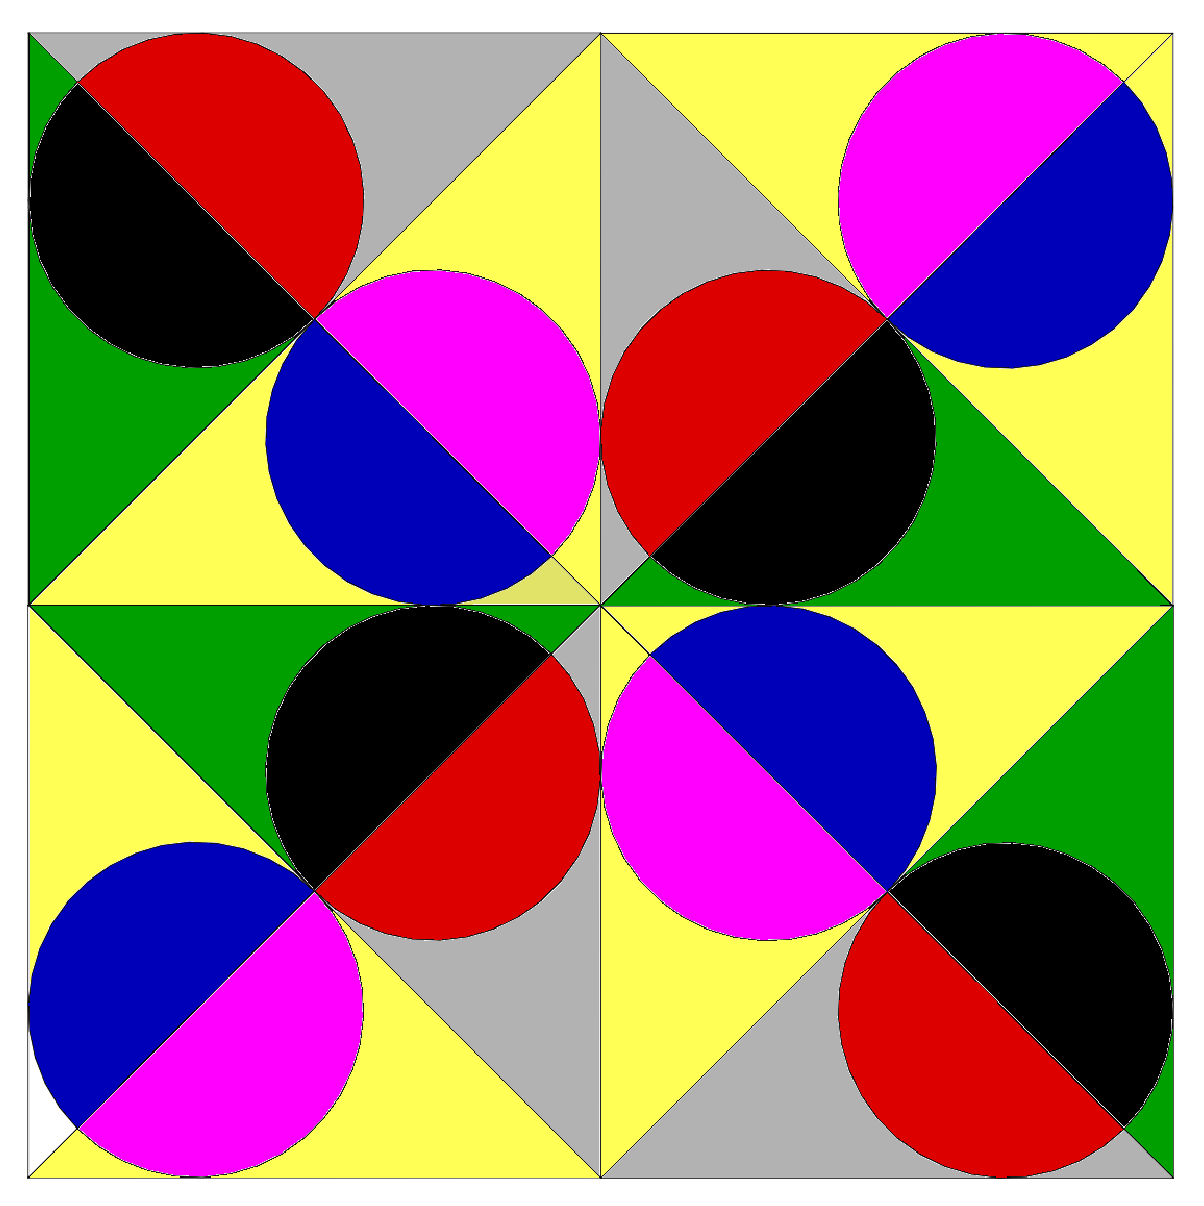
\includegraphics[width=6cm]{Geometrie/Images/G9_ex_rosace}
%\end{minipage}
%\ \\
%\end{corrige}


